\documentclass[letterpaper,11pt]{memoir}
  \usepackage[utf8]{inputenc}
  \usepackage{fourier,microtype}       % texte en Utopia
  \usepackage[scaled=0.82]{beramono}   % code en Bera
  \renewcommand{\sfdefault}{Myriad-LF} % titres en MyriadPro
  \usepackage{natbib,url}
  \usepackage[english,francais]{babel}
  \usepackage[autolanguage]{numprint}
  \usepackage{vgmath,actu,amsmath,amsthm,amsfonts,icomma}
  \usepackage[noae]{Sweave}
  \usepackage{paralist}
  \usepackage[shortlabels]{enumitem}
  \usepackage{textpos}
  \usepackage{graphicx,color,multicol,soulutf8}
  \usepackage{manfnt}                  % \mantriangleright (puce)
  \usepackage{marvosym}                % \Forward et \ForwardToEnd
  \usepackage{listingsutf8,answers}
  \usepackage{pdfpages}                % couvertures
  \usepackage{xr}                      % référence au chap. 3

  %%% Références externes
  \externaldocument{operateurs}

  %%%  Couleurs
  \definecolor{comments}{rgb}{0.7,0,0}
  \definecolor{darkred}{rgb}{0.8,0,0}
  \definecolor{shadecolor}{gray}{0}
  \definecolor{link}{rgb}{0,0,0.4}

  %%% Hyperliens
  \usepackage{hyperref}
  \hypersetup{colorlinks,allcolors=link}

  %%% ============
  %%%  Page titre
  %%% ============
  \title{%
    \fontseries{b}\fontsize{42}{33}\selectfont ACT 2002 \\
    \fontseries{m}\fontsize{32}{33}\selectfont Méthodes numériques \\
                                               en actuariat \\[20mm]
    \fontseries{b}\fontsize{36}{36}\selectfont Partie IV \\
    \fontseries{m}\fontsize{32}{36}\selectfont Algèbre linéaire}
  \author{%
    \fontseries{b}\fontsize{16}{20}\selectfont Vincent Goulet \\
    \fontseries{m}\fontsize{14}{18}\selectfont Professeur titulaire \textbar\
                                               École d'actuariat \textbar\
                                               Université Laval}
  \date{%
    \fontseries{m}\fontsize{14}{18}\selectfont Notes de cours \textbar\
                                               Exercices \textemdash\
                                               édition 2013}

  %%% ===================
  %%%  STYLE DU DOCUMENT
  %%% ===================

  %% Titres des chapitres
  \chapterstyle{hangnum}
  \renewcommand{\chaptitlefont}{\normalfont\Huge\sffamily\bfseries\raggedright}

  %% Marges, entêtes et pieds de page
  \setlength{\marginparsep}{7mm}
  \setlength{\marginparwidth}{13mm}
  \setlength{\headwidth}{\textwidth}
  \addtolength{\headwidth}{\marginparsep}
  \addtolength{\headwidth}{\marginparwidth}

  %% Titres des sections et sous-sections
  \setsecheadstyle{\normalfont\Large\sffamily\bfseries\raggedright}
  \setsubsecheadstyle{\normalfont\large\sffamily\bfseries\raggedright}
  \maxsecnumdepth{subsection}
  \setsecnumdepth{subsection}

  %% Listes. Paramétrage avec enumitem.
  \setlist[enumerate]{leftmargin=*,align=left}
  \setlist[enumerate,2]{label=\alph*),labelsep=*,leftmargin=1.5em}
  \setlist[enumerate,3]{label=\roman*),labelsep=0.5em,align=right}
  \setlist[itemize]{leftmargin=*,align=left}

  %% Noms de fonctions, code, etc.
  \newcommand{\code}[1]{\texttt{#1}}
  \newcommand{\pkg}[1]{\textbf{#1}}

  %% Environnements d'exemples et al.
  \theoremstyle{plain}
  \newtheorem{algorithme}{Algorithme}[chapter]
  \newtheorem{thm}{Théorème}[chapter]

  \theoremstyle{definition}
  \newtheorem{exemple}{Exemple}[chapter]
  \newtheorem{definition}{Définition}[chapter]
  \newtheorem*{astuce}{Astuce}

  \theoremstyle{remark}
  \newtheorem*{remarque}{Remarque}
  \newtheorem*{remarques}{Remarques}
  \newenvironment{rem}{\begin{remarque} \mbox{}}{\end{remarque}}
  \newenvironment{rems}{\begin{remarques} \mbox{}}{\end{remarques}}

  %% Options de babel
  \frenchbsetup{CompactItemize=false,%
    ThinSpaceInFrenchNumbers=true,
    ItemLabeli=\mantriangleright,
    ItemLabelii=\textendash}
  \addto\captionsfrench{\def\figurename{{\scshape Fig.}}}
  \addto\captionsfrench{\def\tablename{{\scshape Tab.}}}

  %%% =========================
  %%%  Nouveaux environnements
  %%% =========================

  %% Listes d'objectifs au début des chapitres
  \newenvironment{objectifs}{%
    \noindent
    \begin{framed}
      \vspace{-1.33\baselineskip}
      \begin{shaded}
        \noindent\sffamily\bfseries\textcolor{white}{Objectifs du chapitre}
      \end{shaded}
      \vspace{-0.6\baselineskip}
      \begin{itemize}[nosep]
        \small}
      {\end{itemize}
    \end{framed}}

  %% Environnements de Sweave
  \DefineVerbatimEnvironment{Sinput}{Verbatim}{xleftmargin=\parindent}
  \DefineVerbatimEnvironment{Soutput}{Verbatim}{xleftmargin=\parindent}
  \DefineVerbatimEnvironment{Scode}{Verbatim}{xleftmargin=\parindent}
  \fvset{listparameters={\setlength{\topsep}{0pt}}}
  \renewenvironment{Schunk}{\vspace{\topsep}}{\vspace{\topsep}}

  %% Exercices et réponses
  \Newassociation{sol}{solution}{solutions}
  \Newassociation{rep}{reponse}{reponses}
  \newcounter{exercice}[chapter]
  \newenvironment{exercice}{%
    \begin{list}{\bfseries \thechapter.\arabic{exercice}}{%
        \refstepcounter{exercice}
        \settowidth{\labelwidth}{\bfseries \thechapter.\arabic{exercice}}
        \setlength{\leftmargin}{\labelwidth}
        \addtolength{\leftmargin}{\labelsep}
        \setlist[enumerate,1]{label=\alph*),labelsep=*,leftmargin=1.5em}
        \setlist[enumerate,2]{label=\roman*),labelsep=0.5em,align=right}}
      \item}
    {\end{list}}
  \renewenvironment{reponse}[1]{%
    \begin{enumerate}[label=\textbf{#1}]
      \item}
    {\end{enumerate}}
  \renewcommand{\reponseparams}{{\thechapter.\theexercice}}
  \renewenvironment{solution}[1]{%
    \begin{enumerate}[label=\textbf{#1}]
      \item}
    {\end{enumerate}}
  \renewcommand{\solutionparams}{{\thechapter.\theexercice}}

  %%% Changements au fil de la lecture
  \newenvironment{gotoR}{%
    \begin{framed}%
      \noindent
      \begin{minipage}{0.07\linewidth}
        \raisebox{-0.5em}[0em][0em]{\LARGE\ForwardToEnd}
      \end{minipage}
      \begin{minipage}[t]{0.88\linewidth}}
      {\end{minipage}%
    \end{framed}}

  \newenvironment{dansR}{%
    \begin{framed}%
      \noindent
      \begin{minipage}{0.07\linewidth}
        \raisebox{-0.5em}[0em][0em]{\LARGE\sffamily R}
      \end{minipage}
      \begin{minipage}[t]{0.88\linewidth}}
      {\end{minipage}%
    \end{framed}}


  %%% Remarques importantes
  \newenvironment{important}{%
    \begin{framed}%
      \noindent
      \begin{minipage}{0.1\linewidth}
        \raisebox{-0.5em}[0em][0em]{\LARGE\danger}
      \end{minipage}
      \begin{minipage}[t]{0.85\linewidth}}
      {\end{minipage}%
    \end{framed}}

  %%% =============================================
  %%%  Paramètres pour les sections de code source
  %%% =============================================
  \lstloadlanguages{R}
  \lstset{language=R,
    extendedchars=true,
    inputencoding=utf8/latin1,
    basicstyle=\small\ttfamily,
    commentstyle=\color{comments}\slshape,
    keywordstyle=\mdseries,
    showstringspaces=false}

  %%% =====================
  %%%  Nouvelles commandes
  %%% =====================
  \newcommand{\R}{\mathbb{R}}
  \newcommand{\tr}{\mathrm{tr}}

  %%% Indications de capsule vidéo
  \setul{1.5pt}{0.7pt}
  \newcommand{\video}{%
    $\mathrel{\vcenter{\offinterlineskip%
        \fontsize{32}{32}\selectfont
        \hbox{$\bigcirc$}%
        \fontsize{24}{22}\selectfont\vskip-20.4pt\hskip8.5pt
        \hbox{\Forward}}}$}
  \newcommand{\capsule}[1]{\marginpar{\video}\ul{#1}}

  %%% Support pour sous-tableaux et sous-figures
  \newsubfloat{figure}

  %%% Style de la bibliographie
  \bibliographystyle{francais}

  %%% Numérotation des chapitres
  \setcounter{chapter}{12}

  %% Longueur utilisée dans les solutions d'algèbre
  %% linéaire.
  \newlength{\ocolumnsep}

  %% Aide pour la césure
  \hyphenation{cons-tante}

%  \includeonly{pagegarde,notices}

\begin{document}

\frontmatter

\pagestyle{empty}

%% Page couverture avant. Il faut modifier la largeur des graphiques
%% puisque Sweave la règle à 0.8\textwidth.
\setkeys{Gin}{width=\paperwidth}
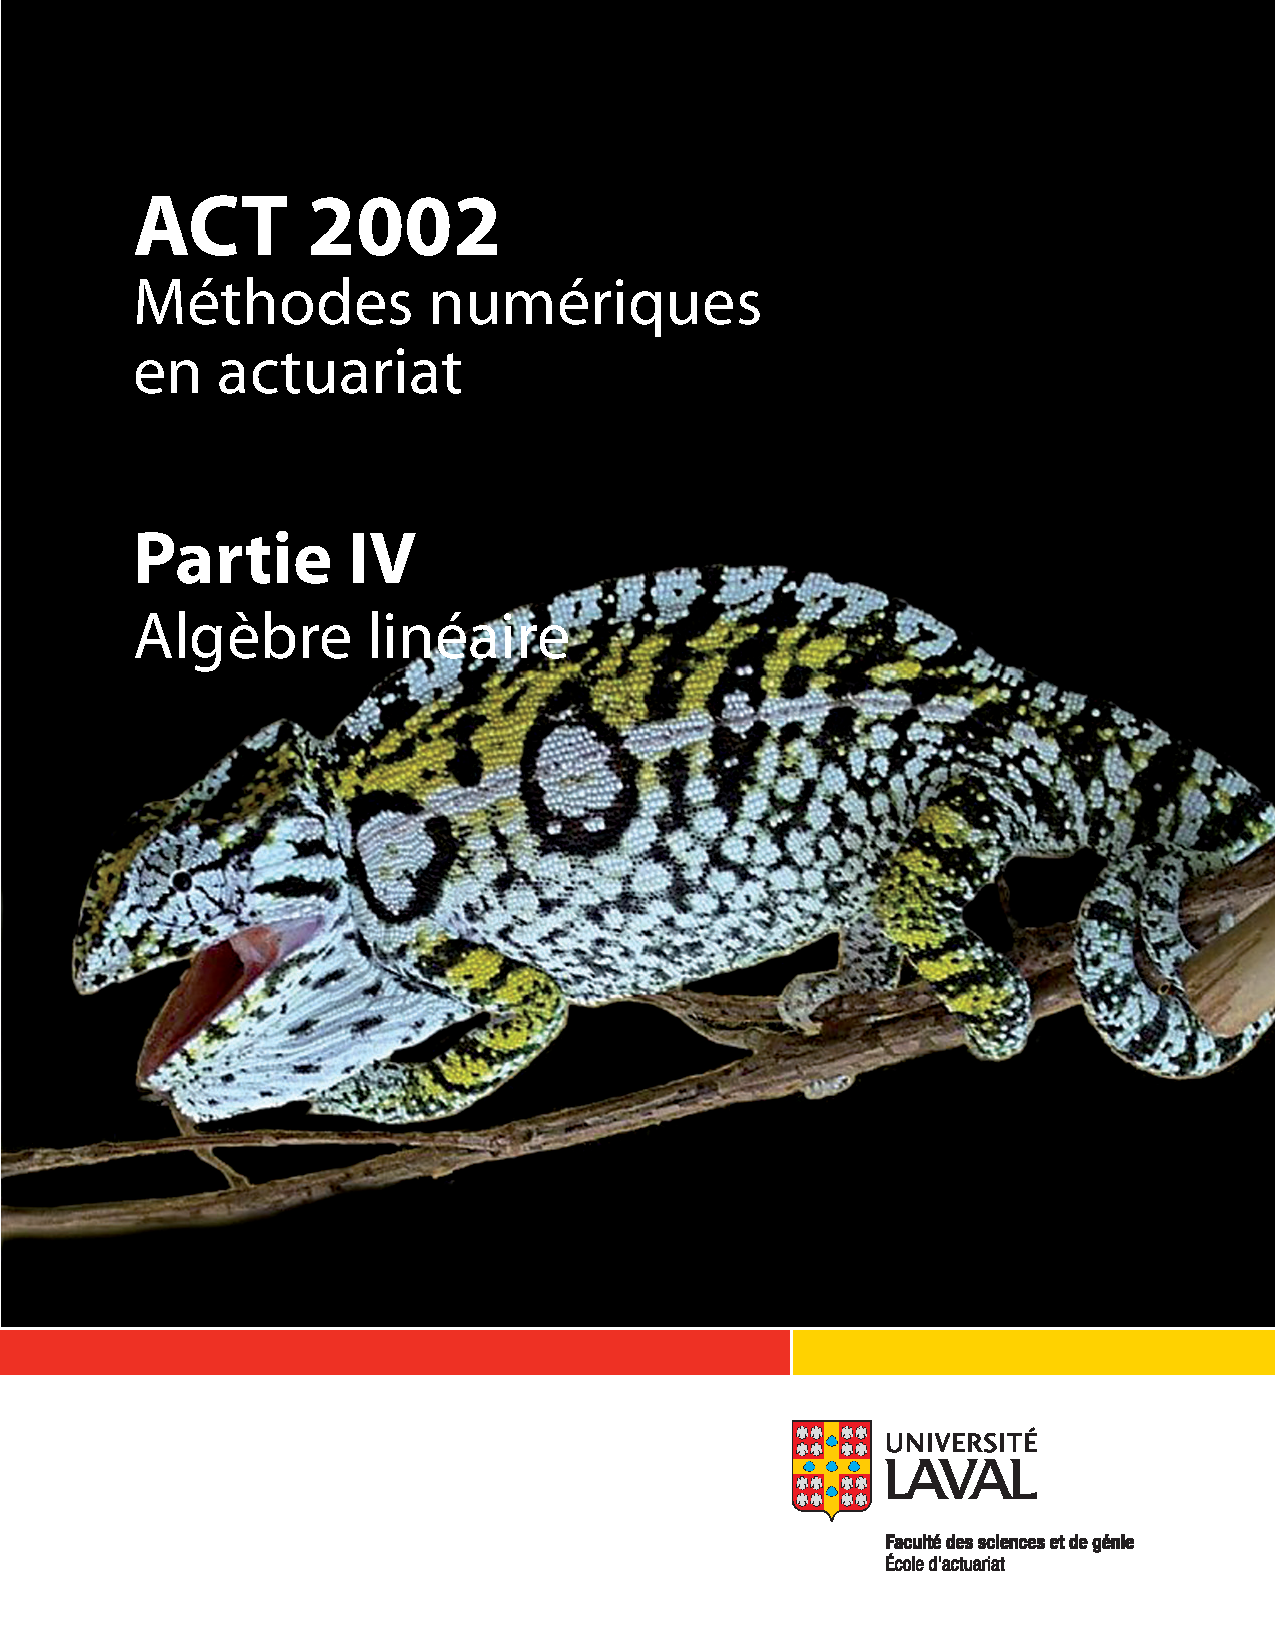
\includepdf[pages=1]{couvertures-partie_4}
\setkeys{Gin}{width=0.8\textwidth}
\cleardoublepage

\begin{adjustwidth*}{-12mm}{-72mm}
  \sffamily
  \raggedright
  \vspace*{-17mm}
  \thetitle \\
  \vspace*{20mm}
  \theparttitle \\
  \vspace*{32mm}
  \theauthor \\
  \vspace*{\fill}
  \thedate
\end{adjustwidth*}

%%% Local Variables:
%%% mode: latex
%%% TeX-master: "methodes_numeriques-partie_3"
%%% coding: utf-8
%%% End:

\clearpage

\begingroup
\calccentering{\unitlength}
\begin{adjustwidth*}{\unitlength}{-\unitlength}
  \setlength{\parindent}{0pt}
  \setlength{\parskip}{\baselineskip}

  {\textcopyright} {\year} Vincent Goulet \\

  
\includegraphics[height=7mm,keepaspectratio=true]{../share/by-sa}\\%
Cette création est mise à disposition selon le contrat
\href{http://creativecommons.org/licenses/by-sa/4.0/deed.fr}{%
  Attribution-Partage dans les mêmes conditions 4.0 International} de
Creative Commons. En vertu de ce contrat, vous êtes libre de:
\begin{itemize}
\item \textbf{partager} --- reproduire, distribuer et communiquer
  l'{\oe}uvre;
\item \textbf{remixer} --- adapter l'{\oe}uvre;
\item utiliser cette {\oe}uvre à des fins commerciales.
\end{itemize}
Selon les conditions suivantes:

\begin{tabularx}{\linewidth}{@{}lX@{}}
  \raisebox{-9mm}[0mm][13mm]{%
    
\includegraphics[height=11mm,keepaspectratio=true]{../share/by}} &
  \textbf{Attribution} --- Vous devez créditer l'{\oe}uvre, intégrer
  un lien vers le contrat et indiquer si des modifications ont été
  effectuées à l'{\oe}uvre. Vous devez indiquer ces informations par
  tous les moyens possibles, mais vous ne pouvez suggérer que
  l'Offrant vous soutient ou soutient la façon dont vous avez utilisé
  son {\oe}uvre. \\
  \raisebox{-9mm}{
\includegraphics[height=11mm,keepaspectratio=true]{../share/sa}}
  & \textbf{Partage dans les mêmes conditions} --- Dans le cas où vous
  modifiez, transformez ou créez à partir du matériel composant
  l'{\oe}uvre originale, vous devez diffuser l'{\oe}uvre modifiée dans
  les même conditions, c'est à dire avec le même contrat avec lequel
  l'{\oe}uvre originale a été diffusée.
\end{tabularx}


  \textbf{Code source} \\
  Le code source {\LaTeX} et R de ce document est disponible à l'adresse
    \url{https://svn.fsg.ulaval.ca/svn-pub/vgoulet/documents/methodes_numeriques/}
  ou en communiquant directement avec l'auteur.

  \textbf{Couverture} \\
  Le reptile en couverture est un caméléon tapis (\emph{Furcifer
    lateralis}) originaire de Madagascar. Adulte, sa taille atteint
  les 25~cm, queue comprise.

  Crédit photo: Michabln Schwarz; \url{http://fc-foto.de/2077174}
\end{adjustwidth*}
\endgroup

%%% Local Variables:
%%% mode: latex
%%% TeX-master: "methodes_numeriques-partie_4"
%%% coding: utf-8
%%% End:

\clearpage

\pagestyle{companion}

\chapter*{Introduction}
\addcontentsline{toc}{chapter}{Introduction}
\markboth{Introduction}{Introduction}

La simulation stochastique est une technique utilisée dans un grand
nombre de domaines. On n'a qu'à penser aux simulations boursières qui
font l'objet d'un concours annuel, aux voitures qui sont d'abord
conçues sur ordinateur et soumises à des tests de collision virtuels,
ou encore aux prévisions météo qui ne en fait les résultats de
simulations de systèmes climatiques d'une grande complexité.

Toute simulation stochastique repose sur une source de nombres
aléatoires de qualité. Comment en générer un grand nombre rapidement
et, surtout, comment s'assurer que les nombres produits sont bien
aléatoires? C'est un sujet d'une grande importance, mais aussi fort
complexe. Nous nous contenterons donc de l'effleurer en étudiant les
techniques de base dans le \autoref{chap:generation}.

En actuariat, nous avons habituellement besoin de nombres aléatoires
provenant d'une loi de probabilité non uniforme. Le
\autoref{chap:simulation} présente quelques algorithmes pour
transformer des nombres aléatoires uniformes en nombres non uniformes.
Évidemment, des outils informatiques sont aujourd'hui disponibles pour
générer facilement et rapidement des nombres aléatoires de diverses
lois de probabilité. Nous passons en revue les fonctionnalités de R et
de Excel à ce chapitre.

Enfin, cette partie du cours se termine au
\autoref{chap:montecarlo} par une application à première vue
inusitée de la simulation, soit le calcul d'intégrales définies par la
méthode dite Monte Carlo.

Chaque chapitre propose un problème à résoudre au fil du texte.
L'énoncé du problème, les indications en cours de chapitre et la
solution complète se présentent dans des encadrés de couleur
contrastante et marqués des symboles {\faCogs}, {\faBolt} et
{\faLightbulbO}.

L'étude de ce document implique quelques allers-retours entre le texte
et les sections de code informatique présentes dans chaque chapitre.
Les sauts vers ces sections sont clairement indiqués dans le texte par
des mentions mises en évidence par le symbole {\faFastForward}.

Les fichiers de code informatique des sections d'exemples sont
disponibles dans le %
\href{http://libre.act.ulaval.ca/}{Portail libre} %
de l'École d'actuariat. On peut y accéder facilement en suivant le
lien fourni à la page précédente.

Un symbole de lecture vidéo dans la marge indique qu'une capsule vidéo
est disponible dans la %
\capsule{http://www.youtube.com/user/VincentGouletACT2002}{chaîne
  YouTube} %
du cours sur le sujet en hyperlien.

Tous les chapitres comportent des exercices. Les réponses de ceux-ci se
retrouvent à la fin de chacun des chapitres et les solutions complètes,
en annexe. En consultation électronique, le numéro d'un exercice est
un hyperlien vers sa solution, et vice versa.

On trouvera également en annexe un bref exposé sur la planification
d'une simulation en R et des rappels sur la transformation de
variables aléatoires.

Je tiens à souligner la précieuse collaboration de MM.~Mathieu
Boudreault, Sébastien Auclair et Louis-Philippe Pouliot lors de la
rédaction des exercices et des solutions. Je remercie également
Mmes~Marie-Pier Laliberté et Véronique Tardif pour l'infographie des
pages couvertures.

%%% Local Variables:
%%% mode: latex
%%% TeX-master: "methodes_numeriques-partie_2"
%%% End:

\cleartorecto
\tableofcontents*

\mainmatter

%% Vignette tirée de xkcd.com
\pagestyle{empty}
\begin{vplace}[0.45]
  \centering
  \setkeys{Gin}{width=\textwidth}
  \begin{minipage}{400pt}
    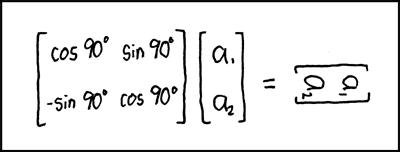
\includegraphics{xkcd.png} \\
    \footnotesize\sffamily%
    Tiré de \href{http://xkcd.com/184/}{XKCD.com}
  \end{minipage}
  \setkeys{Gin}{width=0.8\textwidth}
\end{vplace}
\cleardoublepage

\pagestyle{companion}

\chapter{Révision d'algèbre linéaire}
\label{chap:revision}

%%%
%%% Fichers de solutions et de réponses
%%%

\Opensolutionfile{reponses}[reponses-revision_algebre_lineaire]
\Opensolutionfile{solutions}[solutions-revision_algebre_lineaire]

\begin{Filesave}{reponses}
\section*{Chapitre \ref{chap:revision}}
\addcontentsline{toc}{section}{Chapitre \protect\ref{chap:revision}}

\end{Filesave}

\begin{Filesave}{solutions}
\chapter{Révision d'algèbre linéaire}

\end{Filesave}

%%%
%%% Début des exercices
%%%

\begin{exercice}
  Pour chaque cas ci-dessous, supposer que la matrice donnée est
  une matrice augmentée d'un système d'équations linéaires exprimée
  sous forme échelonnée. Résoudre le système d'équations.
  \begin{enumerate}
    \begin{multicols}{2}
    \item $%
      \begin{bmatrix}
        1 & -3 & 4 & 7 \\
        0 & 1 & 2 & 2 \\
        0 & 0 & 1 & 5
      \end{bmatrix}$
    \item $%
      \begin{bmatrix}
        1 & 0 & 8 & -5 & 6 \\
        0 & 1 & 4 & -9 & 3 \\
        0 & 0 & 1 & 1 & 2
      \end{bmatrix}$
    \end{multicols}
    \begin{multicols}{2}
    \item $%
      \begin{bmatrix}
        1 & 7 & -2 & 0 & -8 & -3 \\
        0 & 0 & 1 & 1 & 6 & 5 \\
        0 & 0 & 0 & 1 & 3 & 9 \\
        0 & 0 & 0 & 0 & 0 & 0
      \end{bmatrix}$
      \columnbreak
    \item $%
      \begin{bmatrix}
        1 & -3 & 7 & 1 \\
        0 & 1 & 4 & 0 \\
        0 & 0 & 0 & 1
      \end{bmatrix}$
    \end{multicols}
  \end{enumerate}
  \begin{sol}
    \begin{enumerate}
    \item On a une solution unique. Le système d'équations
      correspondant est
      \begin{align*}
        x_1 - 3 x_2 + 4 x_3 &= 7 \\
        x_2 + 2 x_3 &= 2 \\
        x_3 &= 5.
      \end{align*}
      Par substitution successive, on obtient $x_3 = 5$, $x_2 = 2 - 2(5)
      = -8$ et $x_1 = 7 + (3)(-8) - 4(5) = -37$.
    \item Le système est sous-déterminé: il compte plus d'inconnues
      que d'équations. Il y a donc une infinité de solutions. Le
      système d'équations correspondant est
      \begin{align*}
        x_1 + 8 x_3 - 5 x_3 &= 6 \\
        x_2 + 4 x_3 - 9 x_4 &= 3 \\
        x_3 + x_4 &= 2.
      \end{align*}
      On utilise la variable libre $x_4 = t$. Ainsi, la solution
      générale du système d'équations est $x_3 = 2 - t$, $x_2 = 3 -
      4(2 - t) + 9t = -5 + 13t$ et $x_1 = 6 - 8 (2 - t) + 5 t = -10 +
      13t$.
    \item On avait à l'origine un système d'équations à quatre
      équations et cinq inconnues. La matrice échelonnée contient une
      ligne complète de zéros, ce qui indique que la quatrième
      équation était une combinaison linéaire des trois autres. Ne
      reste donc qu'un système sous-déterminé à trois équations et
      cinq inconnues:
      \begin{align*}
        x_1 + x_2 - 2 x_3 - 8 x_5 &= -3 \\
        x_3 + x_4 + 6 x_5 &= 5 \\
        x_4 + 3 x_5 &= 9.
      \end{align*}
      Ce système a une infinité de solutions et il faudra, pour les
      exprimer, poser deux variables libres. Les candidates sont les
      variables correspondant aux colonnes sans un 1 sur la diagonale.
      On pose donc $x_2 = s$ et $x_5 = t$. On a alors $x_4 = 9 - 3t$,
      $x_3 = 5 - (9 - 3t) - 6 t = -4 - 3t$ et $x_1 = -3 - 7s + 2 (-4 -
      3t) + 8 t = -11 - 7s + 2t$.
    \item La dernière ligne de la matrice échelonnée correspond à
      l'équation impossible à satisfaire
      \begin{displaymath}
        0 x_1 + 0 x_2 + 0 x_3 = 1,
      \end{displaymath}
      d'où le système n'a pas de solution.
    \end{enumerate}
  \end{sol}
  \begin{rep}
    \begin{enumerate}
    \item $x_1 = -37$, $x_2 = -8$, $x_3 = 5$
    \item $x_1 = -10 + 13t$, $x_2 = -5 + 13t$, $x_3 = 2 - t$, $x_4 =
      t$
    \item $x_1 = -11 - 7s + 2t$, $x_2 = s$, $x_3 = -4 - 3t$, $x_4 = 9 -
      3t$, $x_5 = t$
    \item pas de solution
    \end{enumerate}
  \end{rep}
\end{exercice}

\begin{exercice}
  \label{ex:reduction}
  Résoudre chacun des systèmes d'équations suivants par
  l'élimination gaussienne et l'élimination de Gauss--Jordan.
  \begin{enumerate}
    \begin{multicols}{2}
    \item $%
      \begin{array}[t]{*{2}{r@{\;}c@{\;}}r@{\;=\;}r}
        x_1 &+&  x_2 &+& 2x_3 &  8 \\
        -x_1 &-& 2x_2 &+& 3x_3 &  1 \\
        3x_1 &-& 7x_2 &+& 4x_3 & 10
      \end{array}$
    \item $%
      \begin{array}[t]{*{2}{r@{\;}c@{\;}}r@{\;=\;}r}
        2x_1 &+& 2x_2 &+& 2x_3 &  0 \\
        -2x_1 &+& 5x_2 &+& 2x_3 &  1 \\
        8x_1 &+&  x_2 &+& 4x_3 & -1
      \end{array}$
    \end{multicols}
    \begin{multicols}{2}
    \item $%
      \begin{array}[t]{*{3}{r@{\;}c@{\;}}r@{\;=\;}r}
        x &-&  y &+& 2z &-&  w & -1 \\
        2x &+&  y &-& 2z &-& 2w & -2 \\
        -x &+& 2y &-& 4z &+&  w & 1 \\
        3x & &    & &    &-& 3w & -3
      \end{array}$
    \item $%
      \begin{array}[t]{*{2}{r@{\;}c@{\;}}r@{\;=\;}r}
        &-& 2b &+& 3c & 1 \\
        3a &+& 6b &-& 3c & -2 \\
        6a &+& 6b &+& 3c & 5
      \end{array}$
    \end{multicols}
  \end{enumerate}
  \begin{sol}
    \begin{enumerate}
    \item On donne la solution pour l'élimination gaussienne
      seulement. La matrice augmentée est
      \begin{displaymath}
        \begin{bmatrix}
           1 &  1 &  2 &  8 \\
          -1 & -2 &  3 &  1 \\
           3 & -7 &  4 & 10
         \end{bmatrix}.
      \end{displaymath}
      Les opérations élémentaires à effectuer sur cette matrice pour
      l'exprimer sous forme échelonnée sont, dans l'ordre:
      \begin{enumerate}[1.]
      \item additionner la première ligne à la seconde;
      \item additionner $-3$ fois la première ligne à la troisième;
      \item additionner $-3$ fois la première ligne à la troisième;
      \item multiplier la deuxième ligne par $-1$;
      \item additionner $10$ fois la deuxième ligne à la troisième;
      \item diviser la troisième ligne par $-52$.
      \end{enumerate}
      On obtient alors la matrice échelonnée
      \begin{displaymath}
        \begin{bmatrix}
          1 &  1 &  2 &  8 \\
          0 &  1 & -5 & -9 \\
          0 &  0 &  1 &  2
         \end{bmatrix},
      \end{displaymath}
      d'où $x_3 = 2$, $x_2 = -9 + 5(2) = 1$ et $x_1 = 8 - 1 - 2(2) =
      3$.
    \item On donne la solution pour l'élimination de Gauss--Jordan
      seulement. La matrice augmentée est
      \begin{displaymath}
        \begin{bmatrix}
           2 &  2 &  2 &  0 \\
          -2 &  5 &  2 &  1 \\
           8 &  1 &  4 & -1
         \end{bmatrix}.
      \end{displaymath}
      Les opérations élémentaires à effectuer sur cette matrice pour
      l'exprimer sous forme échelonnée réduite sont les suivantes:
      \begin{enumerate}[1.]
      \item multiplier la première ligne par $\frac{1}{2}$;
      \item additionner 2 fois la première ligne à la deuxième;
      \item additionner $-8$ fois la première ligne à la troisième;
      \item additionner la deuxième ligne à la troisième;
      \item multiplier la deuxième ligne par $\frac{1}{7}$;
      \item additionner $-1$ fois la deuxième ligne à la première.
      \end{enumerate}
      On obtient alors la matrice échelonnée réduite
      \begin{displaymath}
        \begin{bmatrix}
           1 &  0 & 3/7 & -1/7 \\
           0 &  1 & 4/7 & 1/7 \\
           0 &  0 &   0 &   0
         \end{bmatrix}.
      \end{displaymath}
      En posant $x_3 = t$, on a la solution générale $x_2 =
      \frac{1}{7} - \frac{4}{7}t$ et $x_1 = -\frac{1}{7} -
      \frac{3}{7}t$.
    \item On donne la solution pour l'élimination gaussienne
      seulement. La matrice augmentée est
      \begin{displaymath}
        \begin{bmatrix}
           1 & -1 &  2 & -1 & -1 \\
           2 &  1 & -2 & -2 & -2 \\
          -1 &  2 & -4 &  1 &  1 \\
           3 &  0 &  0 & -3 & -3
         \end{bmatrix}.
      \end{displaymath}
      Les opérations élémentaires à effectuer sur cette matrice pour
      l'exprimer sous forme échelonnée sont, dans l'ordre:
      \begin{enumerate}[1.]
      \item additionner $-2$ fois la première ligne à la seconde;
      \item additionner la première ligne à la troisième;
      \item additionner $-3$ fois la première ligne à la quatrième;
      \item additionner $-1$ fois la deuxième ligne à la quatrième;
      \item multiplier la deuxième ligne par $\frac{1}{3}$;
      \item additionner $-1$ fois la deuxième ligne à la troisième.
      \end{enumerate}
      On obtient alors la matrice échelonnée
      \begin{displaymath}
        \begin{bmatrix}
           1 & -1 &  2 & -1 & -1 \\
           0 &  1 & -2 &  0 &  0 \\
           0 &  0 &  0 &  0 &  0 \\
           0 &  0 &  0 &  0 &  0
         \end{bmatrix},
      \end{displaymath}
      d'où $x_3 = s$, $x_4 = t$, $x_2 = 2s$ et $x_1 = -1 + 2s - 2s + t
      = -1 + t$.
    \item En échangeant les première et troisième équations, on a la
      matrice augmentée
      \begin{displaymath}
        \begin{bmatrix}
          6 &  6 &  3 &  5 \\
          3 &  6 & -3 & -2 \\
          0 & -2 &  3 &  1
        \end{bmatrix}.
      \end{displaymath}
      Après les opérations élémentaires
      \begin{enumerate}[1.]
      \item multiplier la première ligne par $\frac{1}{6}$;
      \item additionner $-3$ fois la première ligne à la deuxième;
      \item multiplier la deuxième ligne par $\frac{1}{3}$;
      \item additionner 2 fois la deuxième ligne à la troisième,
      \end{enumerate}
      on obtient la matrice échelonnée
      \begin{displaymath}
        \begin{bmatrix}
          1 &  1 &  1/2 &  5/6 \\
          0 &  1 & -3/2 & -3/2 \\
          0 &  0 &    0 &   -2
        \end{bmatrix}.
      \end{displaymath}
      La troisième équation étant impossible à satisfaire, le système
      n'a pas de solution.
    \end{enumerate}
  \end{sol}
  \begin{rep}
    \begin{enumerate}
    \item $x_1 = 3$, $x_2 = 1$, $x_3 = 2$
    \item $x_1 = -\frac{1}{7} - \frac{3}{7}t$,
          $x_2 = \frac{1}{7} -  \frac{4}{7}t$,
          $x_3 = t$
    \item $x_1 = t - 1$, $x_2 = 2s$, $x_3 = s$, $x_4 = t$
    \item pas de solution
    \end{enumerate}
  \end{rep}
\end{exercice}

\begin{exercice}
  Résoudre chacun des systèmes d'équations suivants par l'élimination
  gaussienne et l'élimination de Gauss--Jordan.
  \begin{enumerate}
    \begin{multicols}{2}
    \item $%
      \begin{array}[t]{*{2}{r@{\;}c@{\;}}r@{\;=\;}r}
        5x_1 &-& 2x_2 &+& 6x_3 & 0 \\
        -2x_1 &+&  x_2 &+& 3x_3 & 1
      \end{array}$
    \item $%
      \begin{array}[t]{*{3}{r@{\;}c@{\;}}r@{\;=\;}r}
        x_1 &-&  2x_2 &+&   x_3 &-&  4x_4 & 1 \\
        x_1 &+&  3x_2 &+&  7x_3 &+&  2x_4 & 2 \\
        x_1 &-& 12x_2 &-& 11x_3 &-& 16x_4 & 5
      \end{array}$
    \end{multicols}
    \begin{multicols}{2}
    \item $%
      \begin{array}[t]{*{4}{r@{\;}c@{\;}}r@{\;=\;}r}
        & &    & &  w &+& 2x &-&  y & 4 \\
        & &    & &    & &  x &-&  y & 3 \\
        & &    & &  w &+& 3x &-& 2y & 7 \\
        2u &+& 4v &+&  w &+& 7x & &    & 7
      \end{array}$
    \end{multicols}
  \end{enumerate}
  \begin{sol}
    La procédure de réduction des matrices augmentées sous forme
    échelonnée est similaire à celle utilisée dans les solutions de
    l'exercice \ref{ex:reduction}. On ne donne, ici que les résultats
    de cette procédure.
    \begin{enumerate}
    \item La matrice échelonnée est
      \begin{displaymath}
        \begin{bmatrix}
          1 & -2/5 & 6/5 & 0 \\
          0 &    1 &  27 & 5
        \end{bmatrix}
      \end{displaymath}
      et la matrice échelonnée réduite est
      \begin{displaymath}
        \begin{bmatrix}
          1 & 0 & 12 & 2 \\
          0 & 1 & 27 & 5
        \end{bmatrix}.
      \end{displaymath}
      Par conséquent, la solution générale est $x_3 = t$, $x_2 = 5 -
      27t$ et $x_1 = 2 - 12t$.
    \item La matrice échelonnée réduite est
      \begin{displaymath}
        \begin{bmatrix}
          1 & -2 &   1 &  -4 & 1 \\
          0 &  1 & 6/5 & 6/5 & 1/5 \\
          0 &  0 &   0 &   0 &   6
        \end{bmatrix}.
      \end{displaymath}
      Ce système n'a donc pas de solution.
    \item La matrice échelonnée est
      \begin{displaymath}
        \begin{bmatrix}
          1 & 2 & 1/2 & 7/2 &  0 & 7/2 \\
          0 & 0 &   1 &   2 & -1 &   4 \\
          0 & 0 &   0 &   1 & -1 &   3 \\
          0 & 0 &   0 &   0 &  0 &   0
        \end{bmatrix}
      \end{displaymath}
      et la matrice échelonnée réduite est
      \begin{displaymath}
        \begin{bmatrix}
          1 & 2 &   0 &   0 &  3 &  -6 \\
          0 & 0 &   1 &   0 &  1 &  -2 \\
          0 & 0 &   0 &   1 & -1 &   3 \\
          0 & 0 &   0 &   0 &  0 &   0
        \end{bmatrix}.
      \end{displaymath}
      Par conséquent, la solution générale est $v = 2$, $y = t$, $x =
      3 + t$, $w = -2 - t$ et $u = -6 - 3t - 2s$.
    \end{enumerate}
  \end{sol}
  \begin{rep}
    \begin{enumerate}
    \item $x_1 = 2 - 12t$, $x_2 = 5 - 27t$, $x_3 = t$
    \item pas de solution
    \item $u = -2s - 3t - 6$,
          $v = s$,
          $w = -t - 2$,
          $x = t + 3$,
          $y = t$
    \end{enumerate}
  \end{rep}
\end{exercice}

\newpage

\begin{exercice}
  Résoudre les systèmes d'équations homogènes suivants.
  \begin{enumerate}
    \begin{multicols}{2}
    \item $%
      \begin{array}[t]{*{2}{r@{\;}c@{\;}}r@{\;=\;}r}
        2x_1 &+&  x_2 &+& 3x_3 & 0 \\
        x_1 &+& 2x_2 & &      & 0 \\
        & &  x_2 &+&  x_3 & 0
      \end{array}$
    \item $%
      \begin{array}[t]{*{3}{r@{\;}c@{\;}}r@{\;=\;}r}
        3x_1 &+&   x_2 &+&  x_3 &+&  x_4 & 0 \\
        5x_1 &-&   x_2 &+&  x_3 &-&  x_4 & 0
      \end{array}$
    \end{multicols}
    \begin{multicols}{2}
    \item $%
      \begin{array}[t]{*{3}{r@{\;}c@{\;}}r@{\;=\;}r}
        & & 2x &+& 2y &+& 4z & 0 \\
        w & &    &-&  y &-& 3z & 0 \\
        2w &+& 3x &+&  y &+&  z & 0 \\
        -2w &+&  x &+& 3y &-& 2z & 0
      \end{array}$
    \end{multicols}
  \end{enumerate}
  \begin{sol}
    \begin{enumerate}
    \item Après quelques opérations élémentaires sur les lignes de la
      matrice augmentée correspondant à ce système d'équations, on
      obtient
      \begin{displaymath}
        \begin{bmatrix}
          2 & 1 &  3 & 0 \\
          0 & 3 & -3 & 0 \\
          0 & 0 &  6 & 0
        \end{bmatrix},
      \end{displaymath}
      d'où $x_3 = x_2 = x_1 = 0$, soit la solution triviale.
    \item La somme des deux équations donne une nouvelle équation
      $4x_1 + x_3 = 0$, d'où $x_3 = -4 x_1$. De la première équation,
      on a également $x_2 = -3 x_1 - x_3 - x_4 = x_1 - x_4$. En
      posant $x_1 = -s$ et $x_4 = t$, on a la solution générale $x_3
      = 4 s$ et $x_2 = -s - t$. Il y a évidemment de multiples autres
      façons d'exprimer la solution générale en utilisant des
      variables libres différentes.
    \item La matrice échelonnée de ce système d'équations est
      \begin{displaymath}
        \begin{bmatrix}
          1 & 0 & -1 &  -3 \\
          0 & 1 &  1 & 7/3 \\
          0 & 0 &  0 &   1 \\
          0 & 0 &  0 &   1
        \end{bmatrix}.
      \end{displaymath}
      On a donc $z = 0$ et, en posant $y = t$, $x = -t$, $w = t$.
    \end{enumerate}
  \end{sol}
  \begin{rep}
    \begin{enumerate}
    \item solution triviale
    \item $x_1 = -s$, $x_2 = -t - s$, $x_3 = 4s$, $x_4 = t$
    \item $w = t$, $x = -t$, $y = t$, $z = 0$
    \end{enumerate}
  \end{rep}
\end{exercice}

\begin{exercice}
  Pour quelle valeur de $a$ le système d'équations
  \begin{displaymath}
    \begin{array}{*{2}{r@{\;}c@{\;}}r@{\;=\;}l}
       x &+& 2y &-&          3z & 4 \\
      3x &-&  y & &          5z & 2 \\
      4x &+&  y &+& (a^2 - 14)z & a + 2
    \end{array}
  \end{displaymath}
  n'aura-t-il aucune solution? Une seule solution? Une infinité de
  solutions?
  \begin{sol}
    Après des opérations élémentaires sur la matrice augmentée du
    système d'équations, on obtient
    \begin{displaymath}
      \begin{bmatrix}
        1 &  2 &        3 & 4 \\
        0 & -7 &       14 & -10 \\
        0 &  0 & a^2 - 16 & a - 4
      \end{bmatrix}.
    \end{displaymath}
    On constate alors que le système d'équations n'a pas de solution
    si $a^2 - 16 = 0$ et $a - 4 \neq 0$, donc lorsque $a = -4$. En
    revanche, si $a^2 - 16 = 0$ et $a - 4 = 0$, soit lorsque $a = 4$,
    le système a une infinité de solutions. Finalement, si $a^2 - 16
    \neq 0 \Leftrightarrow |a| \neq 4$, le système a une solution
    unique.
  \end{sol}
  \begin{rep}
    Aucune solution: $a = -4$. Une seule solution: $a \neq \pm 4$.
    Infinité de solutions: $a = 4$.
  \end{rep}
\end{exercice}

\begin{exercice}
  Soit les matrices $\mat{A}_{4 \times 5}$, $\mat{B}_{4 \times 5}$,
  $\mat{C}_{5 \times 2}$, $\mat{D}_{4 \times 2}$ et $\mat{E}_{5 \times
    4}$. Lesquelles des expressions matricielles suivantes sont
  définies?  Pour les expressions définies, donner les dimensions de
  la matrice résultante.
  \begin{enumerate}
    \begin{multicols}{4}
    \item $\mat{BA}$
    \item $\mat{AC} + \mat{D}$
    \item $\mat{AE} + \mat{B}$
    \item $\mat{AB} + \mat{B}$
    \end{multicols}
    \vspace{-1.5\baselineskip}
    \begin{multicols}{4}
    \item $\mat{E}(\mat{A} + \mat{B})$
    \item $\mat{E}(\mat{AC})$
    \item $\mat{E}^T \mat{A}$
    \item $(\mat{A}^T + \mat{E})\mat{D}$
    \end{multicols}
  \end{enumerate}
  \begin{sol}
    La somme (ou la différence) entre deux matrices est définie si les
    dimensions des matrices sont identiques. Les dimensions du
    résultat seront les mêmes. Quant au produit, il est défini si le
    nombre de colonnes de la première matrice est égal au nombre de
    lignes de la seconde; le résultat est une matrice dont le nombre
    de lignes est égal à celui de la première matrice et le nombre de
    colonnes à celui de la seconde matrice.
    \begin{enumerate}
    \item Le produit $\mat{B} \mat{A}$ n'est pas défini.
    \item Le résultat de $\mat{A} \mat{C}$ est une matrice $4 \times
      2$, donc l'opération $\mat{A} \mat{C} + \mat{D}$ est définie et
      le résultat est une matrice $4 \times 2$.
    \item Le résultat de $\mat{A} \mat{E}$ est une matrice $4 \times
      4$, donc l'opération $\mat{A} \mat{E} + \mat{B}$ n'est pas
      définie.
    \item Le produit $\mat{A} \mat{B}$ n'est pas défini.
    \item La somme $\mat{A} + \mat{B}$ est définie, tout comme le
      produit $\mat{E}(\mat{A} + \mat{B})$. Le résultat est une
      matrice $5 \times 5$.
    \item Le résultat du produit $\mat{A} \mat{C}$ est une matrice $4
      \times 2$, donc $\mat{E}(\mat{AC})$ est une matrice $5 \times 2$.
    \item Puisque $\mat{E}^T$ est une matrice $4 \times 5$, le produit
      $\mat{E}^T \mat{A}$ n'est pas défini.
    \item Le résultat de $\mat{A}^T + \mat{E}$ est une matrice $5
      \times 4$, donc $(\mat{A}^T + \mat{E}) \mat{D}$ est une matrice
      $5 \times 2$.
    \end{enumerate}
  \end{sol}
  \begin{rep}
    \begin{inparaenum}
    \item non défini
    \item $4 \times 2$
    \item non défini
    \item non défini
    \item $5 \times 5$
    \item $5 \times 2$
    \item non défini
    \item $5 \times 2$
    \end{inparaenum}
  \end{rep}
\end{exercice}

\begin{exercice}
  Soit les matrices
  \begin{align*}
    \mat{A}
    &=
    \begin{bmatrix}
      3 & 0 \\ -1 & 2 \\ 1 & 1
    \end{bmatrix} &
    \mat{B}
    &=
    \begin{bmatrix}
      4 & -1 \\ 0 & 2
    \end{bmatrix} &
    \mat{C}
    &=
    \begin{bmatrix}
      1 & 4 & 2 \\ 3 & 1 & 5
    \end{bmatrix} \\
    \mat{D}
    &=
    \begin{bmatrix}
      1 & 5 & 2 \\ -1 & 0 & 1 \\ 3 & 2 & 4
    \end{bmatrix} &
    \mat{E}
    &=
    \begin{bmatrix}
      6 & 1 & 3 \\ -1 & 1 & 2 \\ 4 & 1 & 3
    \end{bmatrix}.
  \end{align*}
  Calculer les expressions suivantes (lorsque possible).
  \begin{enumerate}
    \begin{multicols}{2}
    \item $\mat{D} + \mat{E}$
    \item $\mat{AB}$
    \end{multicols}
    \vspace{-1.5\baselineskip}
    \begin{multicols}{2}
    \item $(2 \mat{D}^T - \mat{E}) \mat{A}$
    \item $(4 \mat{B}) \mat{C} + 2 \mat{B}$
    \end{multicols}
    \vspace{-1.5\baselineskip}
    \begin{multicols}{2}
    \item $(-\mat{AC})^T + 5 \mat{D}^T$
    \item $(\mat{BA}^T - 2 \mat{C})^T$
    \end{multicols}
    \vspace{-1.5\baselineskip}
    \begin{multicols}{2}
    \item $\mat{B}^T (\mat{CC}^T - \mat{A}^T \mat{A})$
    \item $\mat{D}^T \mat{E}^T - (\mat{ED})^T$
    \end{multicols}
    \vspace{-1.5\baselineskip}
    \begin{multicols}{2}
    \item $\tr(\mat{DD}^T)$
    \item $\tr(4 \mat{E}^T - \mat{D})$
    \end{multicols}
  \end{enumerate}
  \begin{sol}
    \begin{enumerate}
    \item On a
      \begin{displaymath}
        \mat{D} + \mat{E}
        =
        \begin{bmatrix}
          1 & 5 & 2 \\ -1 & 0 & 1 \\ 3 & 2 & 4
        \end{bmatrix} +
        \begin{bmatrix}
          6 & 1 & 3 \\ -1 & 1 & 2 \\ 4 & 1 & 3
        \end{bmatrix}
        =
        \begin{bmatrix}
          7 & 6 & 5 \\ -3 & 1 & 3 \\ 7 & 3 & 7
        \end{bmatrix}
      \end{displaymath}
    \item On a
      \begin{displaymath}
        \mat{A} \mat{B}
        =
        \begin{bmatrix}
          3 & 0 \\ -1 & 2 \\ 1 & 1
        \end{bmatrix}
        \begin{bmatrix}
          4 & -1 \\ 0 & 2
        \end{bmatrix}
        =
        \begin{bmatrix}
          12 & -3 \\ -4 & 5 \\ 4 & 1
        \end{bmatrix}.
      \end{displaymath}
    \item On a
      \begin{align*}
        (2 \mat{D}^T - \mat{E}) \mat{A}
        &=
        \left(
          2
          \begin{bmatrix}
            1 & -1 & 3 \\ 5 & 0 & 2 \\ 2 & 1 & 4
          \end{bmatrix} -
          \begin{bmatrix}
            6 & 1 & 3 \\ -1 & 1 & 2 \\ 4 & 1 & 3
          \end{bmatrix}
        \right)
        \begin{bmatrix}
          3 & 0 \\ -1 & 2 \\ 1 & 1
        \end{bmatrix} \\
        &=
        \left(
          \begin{bmatrix}
            2 & -2 & 6 \\ 10 & 0 & 4 \\ 4 & 2 & 8
          \end{bmatrix} -
          \begin{bmatrix}
            6 & 1 & 3 \\ -1 & 1 & 2 \\ 4 & 1 & 3
          \end{bmatrix}
        \right)
        \begin{bmatrix}
          3 & 0 \\ -1 & 2 \\ 1 & 1
        \end{bmatrix} \\
        &=
        \begin{bmatrix}
          -4 & -3 & 3 \\ 11 & -1 & 2 \\ 0 & 1 & 5
        \end{bmatrix} -
        \begin{bmatrix}
          3 & 0 \\ -1 & 2 \\ 1 & 1
        \end{bmatrix} \\
        &=
        \begin{bmatrix}
          -6 & -3 \\ 36 & 0 \\ 4 & 7
        \end{bmatrix}.
      \end{align*}
    \item On a $(4 \mat{B}) \mat{C} + 2 \mat{B} = 2 \mat{B}(2\mat{C} +
      \mat{I})$. Or la somme entre parenthèses n'est pas définie
      puisque la matrice $\mat{C}$ n'est pas carrée.
    \item On a
      \begin{align*}
        (-\mat{AC})^T + 5 \mat{D}^T
        &=
        \left(
          -
          \begin{bmatrix}
            3 & 0 \\ -1 & 2 \\ 1 & 1
          \end{bmatrix}
          \begin{bmatrix}
            1 & 4 & 2 \\ 3 & 1 & 5
          \end{bmatrix}
        \right)^T + 5
        \begin{bmatrix}
          1 & 5 & 2 \\ -1 & 0 & 1 \\ 3 & 2 & 4
        \end{bmatrix}^T \\
        &=
        \left(
          -
          \begin{bmatrix}
            3 & 12 & 6 \\ 5 & -2 & 8 \\ 4 & 5 & 7
          \end{bmatrix}
        \right)^T +
        \begin{bmatrix}
          5 & -5 & 15 \\ 25 & 0 & 10 \\ 10 & 5 & 20
        \end{bmatrix} \\
        &=
        \begin{bmatrix}
          -3 & -5 & -4 \\ -12 & 2 & -5 \\ -6 & -8 & -7
        \end{bmatrix} +
        \begin{bmatrix}
          5 & -5 & 15 \\ 25 & 0 & 10 \\ 10 & 5 & 20
        \end{bmatrix} \\
        &=
        \begin{bmatrix}
          2 & -10 & 11 \\ 13 & 2 & 5 \\ 4 & -3 & 13
        \end{bmatrix}.
      \end{align*}
    \item On a
      \begin{align*}
        (\mat{BA}^T - 2 \mat{C})^T
        &=
        \left(
          \begin{bmatrix}
            4 & -1 \\ 0 & 2
          \end{bmatrix}
          \begin{bmatrix}
            3 & -1 & 1 \\ 0 & 2 & 1
          \end{bmatrix} -
          \begin{bmatrix}
            2 & 8 & 4 \\ 6 & 2 & 10
          \end{bmatrix}
        \right)^T \\
        &=
        \left(
          \begin{bmatrix}
            12 & -6 & 3 \\ 0 & 4 & 2
          \end{bmatrix} -
          \begin{bmatrix}
            2 & 8 & 4 \\ 6 & 2 & 10
          \end{bmatrix}
        \right)^T \\
        &=
        \begin{bmatrix}
          10 & -6 \\ -14 & 2 \\ -1 & -8
        \end{bmatrix}
      \end{align*}
    \item On a
      \begin{align*}
        \mat{C} \mat{C}^T
        &=
        \begin{bmatrix}
          1 & 4 & 2 \\ 3 & 1 & 5
        \end{bmatrix}
        \begin{bmatrix}
          1 & 3 \\ 4 & 1 \\ 2 & 5
        \end{bmatrix} =
        \begin{bmatrix}
          21 & 17 \\ 17 & 35
        \end{bmatrix} \\
        \intertext{et}
        \mat{A}^T \mat{A}
        &=
        \begin{bmatrix}
          3 & -1 & 1 \\ 0 & 2 & 1
        \end{bmatrix}
        \begin{bmatrix}
          3 & 0 \\ -1 & 2 \\ 1 & 1
        \end{bmatrix} =
        \begin{bmatrix}
          11 & -1 \\ -1 & 5
        \end{bmatrix}, \\
        \intertext{d'où}
        \mat{B}^T (\mat{CC}^T - \mat{A}^T \mat{A})
        &=
        \begin{bmatrix}
          4 & 0 \\ -1 & 2
        \end{bmatrix}
        \begin{bmatrix}
          10 & 18 \\ 18 & 30
        \end{bmatrix} =
        \begin{bmatrix}
          40 & 72 \\ 26 & 42
        \end{bmatrix}
      \end{align*}
    \item On a $\mat{D}^T \mat{E}^T - (\mat{ED})^T = (\mat{ED})^T -
      (\mat{ED})^T = \mat{0}_{3 \times 3}$.
    \item Pour calculer la trace, il suffit de connaître les éléments
      de la diagonale. Or l'élément $d_{ii}$ de $\mat{D}\mat{D}^T$ est
      la somme des carrés des éléments de la ligne $i$ de la matrice
      $\mat{D}$. Par conséquent, $\tr(\mat{D}\mat{D}^T) = (1 + 25 + 4)
      + (1 + 0 + 1) + (9 + 4 + 16) = 61$.
    \item Encore une fois, on se concentre seulement sur les éléments
      de la diagonale de $4 \mat{E}^T - \mat{D}$. La transposée ne
      joue donc aucun rôle, ici. Ainsi, $\tr(4 \mat{E}^T - \mat{D}) =
      (24 - 1) + (4 - 0) + (12 - 4) = 35$.
    \end{enumerate}
  \end{sol}
  \begin{rep}
    \raggedright
    \begin{inparaenum}
    \item $\begin{bmatrix} 7 & 6 & 5 \\ -2 & 1 & 3 \\ 7 & 3 & 7
      \end{bmatrix}$
    \item $\begin{bmatrix} 12 & -3 \\ -4 & 5 \\ 4 & 1 \end{bmatrix}$
    \item $\begin{bmatrix} -6 & -3 \\ 36 & 0 \\ 4 & 7 \end{bmatrix}$
    \item non défini
    \item $\begin{bmatrix} 2 & -10 & 11 \\ 13 & 2 & 5 \\ 4 & -3 & 13
      \end{bmatrix}$
    \item $\begin{bmatrix} 10 & -6 \\ -14 & 2 \\ -1 & -8
      \end{bmatrix}$
    \item $\begin{bmatrix} 40 & 72 \\ 26 & 42 \end{bmatrix}$
    \item $\begin{bmatrix} 0&0&0 \\ 0&0&0 \\ 0&0&0 \end{bmatrix}$
    \item 61
    \item 35
    \end{inparaenum}
  \end{rep}
\end{exercice}

\begin{exercice}
  Démontrer que si $\mat{A}$ et $\mat{B}$ sont deux matrices $n \times
  n$, alors $\tr(\mat{A} + \mat{B}) = \tr({\mat{A}}) +
  \tr({\mat{B}})$, où $\tr(\mat{A}) = \sum_{i=1}^n a_{ii}$.
  \begin{sol}
    Puisque $\tr(\mat{A}) = \sum_{i=1}^n a_{ii}$, alors
    \begin{align*}
      \tr({\mat{A}}) + \tr({\mat{B}})
      &= \sum_{i=1}^n a_{ii} + \sum_{i=1}^n b_{ii} \\
      &= \sum_{i=1}^n (a_{ii} + b_{ii}) \\
      &= \tr(\mat{A} + \mat{B}).
    \end{align*}
  \end{sol}
\end{exercice}

\begin{exercice}
  Une matrice $\mat{A}$ est dite \emph{symétrique} si $\mat{A}^T =
  \mat{A}$ et \emph{antisymétrique} si $\mat{A}^T = - \mat{A}$.
  Démontrer les énoncés suivants, étant donné une matrice carrée
  $\mat{A}$.
  \begin{enumerate}
  \item $\mat{AA}^T$ et $\mat{A}^T\mat{A}$ sont symétriques.
  \item $\mat{A} - \mat{A}^T$ est antisymétrique.
  \end{enumerate}
  \begin{sol}
    \begin{enumerate}
    \item On a que $(\mat{A} \mat{A}^T)^T = (\mat{A}^T)^T \mat{A}^T =
      \mat{A} \mat{A}^T$, d'où $\mat{A} \mat{A}^T$ est symétrique. On
      procède de même pour le second résultat.
    \item On a que $(\mat{A} - \mat{A}^T)^T = \mat{A}^T - \mat{A} =
      -(\mat{A} - \mat{A}^T)$, d'où $\mat{A} - \mat{A}^T$ est
      antisymétrique.
    \end{enumerate}
  \end{sol}
\end{exercice}

\begin{exercice}
  Démontrer que si $\mat{A}^T \mat{A} = \mat{A}$, alors $\mat{A}$
  est symétrique et $\mat{A} = \mat{A}^2$. Une matrice qui satisfait
  cette dernière égalité est dite \emph{idempotente}.
  \begin{sol}
    Tout d'abord, $\mat{A}^T = (\mat{A}^T \mat{A})^T = \mat{A}^T
    \mat{A} = \mat{A}$, d'où $\mat{A}^T \mat{A}$ est symétrique. De
    plus, si $\mat{A}$ est symétrique, alors $\mat{A} = \mat{A}^T
    \mat{A} = \mat{A} \mat{A} = \mat{A}^2$. La matrice $\mat{A}$ est
    donc idempotente.
  \end{sol}
\end{exercice}

\begin{exercice}
  Lesquels des ensembles de vecteurs dans $\R^3$ suivants sont
  linéairement dépendants?
  \begin{enumerate}
  \item $( 4, -1,  2)$, $(-4, 10,  2)$
  \item $(-3,  0,  4)$, $( 5, -1,  2)$, $( 1,  1,  3)$
  \item $( 8, -1,  3)$, $( 4,  0,  1)$
  \item $(-2,  0,  1)$, $( 3,  2,  5)$, $( 6, -1,  1)$, $(7, 0, -2)$
  \end{enumerate}
  \begin{sol}
    Enfin
    \begin{enumerate}
    \item Deux vecteurs de $\mathbb{R}^3$ sont nécessairement
      linéairement indépendants à moins que l'un ne soit un multiple
      de l'autre. Ce n'est pas le cas ici.
    \item Trois vecteurs sont linéairement dépendants si l'un est une
      combinaison linéaire des deux autres. Si c'est le cas, le
      déterminant de la matrice formée des coordonnées des vecteurs
      sera nul. Or, ici,
      \begin{displaymath}
        \begin{vmatrix}
          -3 & 5 & 1 \\ 0 & -1 & 1 \\ 4 & 2 & 3
        \end{vmatrix} = 39 \neq 0.
      \end{displaymath}
      Les vecteurs sont donc linéairement indépendants.
    \item Le second vecteur n'est pas un multiple du premier, donc les
      vecteurs sont linéairement indépendants.
    \item Un ensemble de quatre vecteurs de $\mathbb{R}^3$ est
      nécessairement linéairement dépendant.
    \end{enumerate}
  \end{sol}
  \begin{rep}
    (d) seulement
  \end{rep}
\end{exercice}

\begin{exercice}
  Soit $\mat{v}_1, \mat{v}_2, \mat{v}_3 \in \R^3$. Déterminer si
  les trois vecteurs se trouvent dans un plan.
  \begin{enumerate}
  \item $\mat{v}_1 = ( 2, -2,  0)$,
        $\mat{v}_2 = ( 6,  1,  4)$,
        $\mat{v}_3 = ( 2,  0, -4)$
  \item $\mat{v}_1 = (-6,  7,  2)$,
        $\mat{v}_2 = ( 3,  2,  4)$,
        $\mat{v}_3 = ( 4, -1,  2)$
  \end{enumerate}
  \begin{sol}
    Les trois vecteurs se trouvent dans un plan si seulement deux
    vecteurs sont linéairement indépendants (ceux-ci engendrent un
    plan dont fait alors partie le troisième).
    \begin{enumerate}
    \item Soit la matrice
      \begin{displaymath}
        \mat{A} =
        \begin{bmatrix}
          2 & 6 & 2 \\ -2 & 1 & 0 \\ 0 & 4 & -4
        \end{bmatrix}.
      \end{displaymath}
      En additionnant la première et la deuxième ligne, on obtient
      \begin{displaymath}
        \begin{bmatrix}
          2 & 6 & 2 \\ 0 & 7 & 2 \\ 0 & 4 & -4
        \end{bmatrix}.
      \end{displaymath}
      La troisième ligne n'étant pas un multiple de la deuxième, on
      voit que la seule solution du système d'équations homogène
      $\mat{A} \mat{x} = \mat{0}$ est la solution triviale. Par
      conséquent, les trois vecteurs sont linéairement indépendants et
      ne se trouvent pas dans un plan. On pourrait également vérifier
      que $\det(\mat{A}) \neq 0$.
    \item Soit la matrice
      \begin{displaymath}
        \mat{A} =
        \begin{bmatrix}
          -6 & 3 & 4 \\ 7 & 2 & -1 \\ 2 & 4 & 2
        \end{bmatrix}.
      \end{displaymath}
      À la suite d'opérations élémentaires sur les lignes, on obtient
      \begin{displaymath}
        \begin{bmatrix}
          -6 & 3 & 4 \\ 0 & 3 & 2 \\ 0 & 0 & 0
        \end{bmatrix}.
      \end{displaymath}
      Il n'y a donc que deux vecteurs linéairement indépendants
      formant un plan dans cet ensemble.
    \end{enumerate}
  \end{sol}
  \begin{rep}
    \begin{inparaenum}
    \item non
    \item oui
    \end{inparaenum}
  \end{rep}
\end{exercice}

\begin{exercice}
  \label{ex:inverse_diagonale}
  Soit la matrice
  \begin{displaymath}
    \mat{A} =
    \begin{bmatrix}
      a_{11} &      0 & \cdots &      0 \\
           0 & a_{22} & \cdots &      0 \\
      \vdots & \vdots &        & \vdots \\
           0 &      0 & \cdots & a_{nn}
    \end{bmatrix},
  \end{displaymath}
  où $\prod_{i=1}^n a_{ii} \neq 0$. Démontrer que $\mat{A}$ est
  inversible et trouver son inverse.
  \begin{sol}
    La condition $\prod_{i=1}^n a_{ii} \neq 0$ peut, d'une part,
    signifier que $\det(\mat{A}) \neq 0$ ou, d'autre part, qu'il n'y
    aucun zéro sur la diagonale et, par conséquent, aucune ligne de
    zéros dans la matrice. Dans un cas comme dans l'autre, cela
    signifie que l'inverse existe. En utilisant la technique
    consistant à transformer la matrice $[\mat{A}|\mat{I}]$ en
    $[\mat{I}|\mat{A}^{-1}]$, on voit immédiatement que
    \begin{displaymath}
      \mat{A} =
      \begin{bmatrix}
        a_{11}^{-1} &          0 & \cdots &      0 \\
                 0 & a_{22}^{-1} & \cdots &      0 \\
            \vdots &     \vdots &        & \vdots \\
                 0 &          0 & \cdots & a_{nn}^{-1}
      \end{bmatrix}.
    \end{displaymath}
  \end{sol}
\end{exercice}

\newpage

\begin{exercice}
  Soit les matrices
  \begin{align*}
    \mat{A}
    &=
    \begin{bmatrix}
      3 & 4 & 1 \\ 2 & -7 & -1 \\ 8 & 1 & 5
    \end{bmatrix} &
    \mat{B}
    &=
    \begin{bmatrix}
      8 & 1 & 5 \\ 2 & -7 & -1 \\ 3 & 4 & 1
    \end{bmatrix} &
    \mat{C}
    &=
    \begin{bmatrix}
      3 & 4 & 1 \\ 2 & -7 & -1 \\ 2 & -7 & 3
    \end{bmatrix}.
  \end{align*}
  Trouver les matrices élémentaires $\mat{E}_1$, $\mat{E}_2$ et
  $\mat{E}_3$ satisfaisant les équations suivantes.
  \begin{enumerate}
    \begin{multicols}{4}
    \item $\mat{E}_1 \mat{A} = \mat{B}$
    \item $\mat{E}_2 \mat{B} = \mat{A}$
    \item $\mat{E}_3 \mat{A} = \mat{C}$
    \item $\mat{E}_4 \mat{C} = \mat{A}$
    \end{multicols}
  \end{enumerate}
  \begin{sol}
    Une matrice élémentaire est le résultat d'une opération
    élémentaire sur la matrice identité.
    \begin{enumerate}
    \item On souhaite inverser les première et troisième ligne de la
      matrice $\mat{A}$. Par conséquent,
      \begin{displaymath}
        \mat{E}_1 =
        \begin{bmatrix}
          0 & 0 & 1 \\ 0 & 1 & 0 \\ 1 & 0 & 0
        \end{bmatrix}.
      \end{displaymath}
    \item Même chose que ci-dessus.
    \item La matrice $\mat{C}$ est obtenue à partir de la matrice
      $\mat{A}$ en additionnant $-2$ fois la première ligne à la
      troisième ligne. Par conséquent,
      \begin{displaymath}
        \mat{E}_3 =
        \begin{bmatrix}
          1 & 0 & 0 \\ 0 & 1 & 0 \\ -2 & 0 & 1
        \end{bmatrix}.
      \end{displaymath}
    \item De façon similaire, on obtient la matrice $\mat{A}$ en
      additionnant 2 fois la première ligne de la matrice $\mat{C}$ à
      la troisième ligne. On a donc
      \begin{displaymath}
        \mat{E}_4 =
        \begin{bmatrix}
          1 & 0 & 0 \\ 0 & 1 & 0 \\ 2 & 0 & 1
        \end{bmatrix}.
      \end{displaymath}
    \end{enumerate}
  \end{sol}
  \begin{rep}
    \begin{inparaenum}
    \item $\begin{bmatrix} 0&0&1 \\ 0&1&0 \\ 1&0&0 \end{bmatrix}$
    \item $\begin{bmatrix} 0&0&1 \\ 0&1&0 \\ 1&0&0 \end{bmatrix}$
    \item $\begin{bmatrix} 1&0&0 \\ 0&1&0 \\ -2&0&1 \end{bmatrix}$
    \item $\begin{bmatrix} 1&0&0 \\ 0&1&0 \\ 2&0&1 \end{bmatrix}$
    \end{inparaenum}
  \end{rep}
\end{exercice}

\begin{exercice}
  \label{ex:inverse_par_op_elementaires}
  Utiliser la méthode de l'exemple
  \ref{ex:revision:inverse_par_op_elementaires} des notes de cours
  (opérations élémentaires sur les lignes) pour trouver l'inverse des
  matrices suivantes, si elle existe. Le cas échéant, vérifier votre
  réponse par multiplication de la matrice et de son inverse.
  \begin{enumerate}
    \begin{multicols}{3}
    \item $%
      \begin{bmatrix}
        3 & 4 & -1 \\ 1 & 0 & 3 \\ 2 & 5 & -4
      \end{bmatrix}$
    \item $%
      \begin{bmatrix}
        -1 & 3 & -4 \\ 2 & 4 & 1 \\ -4 & 2 & -9
      \end{bmatrix}$
    \item $%
      \begin{bmatrix}
        1 & 0 & 1 \\ 0 & 1 & 1 \\ 1 & 1 & 0
      \end{bmatrix}$
    \end{multicols}
    \begin{multicols}{3}
    \item $%
      \begin{bmatrix}
        2 & 6 & 6 \\ 2 & 7 & 6 \\ 2 & 7 & 7
      \end{bmatrix}$
    \item $%
      \begin{bmatrix}
        1 & 0 & 1 \\ -1 & 1 & 1 \\ 0 & 1 & 0
      \end{bmatrix}$
    \end{multicols}
  \end{enumerate}
  \begin{sol}
    Par des opérations élémentaire sur les lignes, on cherche à
    transformer la matrice $[\mat{A}|\mat{I}]$ en
    $[\mat{I}|\mat{A}^{-1}]$. Ci-dessous, $L_i$ identifie la ligne $i$
    d'une matrice, le symbole $\leftarrow$ signifie qu'une ligne est
    remplacée et le symbole $\leftrightarrow$ que deux lignes sont
    échangées.
    \begin{enumerate}
    \item
      \begin{multicols}{2}
        Matrice de départ \\
        \columnbreak
        $%
        \left[
          \begin{array}{rrr|rrr}
            3 & 4 & -1 & 1 & 0 & 0 \\
            1 & 0 &  3 & 0 & 1 & 0 \\
            2 & 5 & -4 & 0 & 0 & 1
          \end{array}
        \right]
        $
      \end{multicols}
      \begin{multicols}{2}
        $L_1 \leftrightarrow L_2$ \\
        \columnbreak
        $%
        \left[
          \begin{array}{rrr|rrr}
            1 & 0 &  3 & 0 & 1 & 0 \\
            3 & 4 & -1 & 1 & 0 & 0 \\
            2 & 5 & -4 & 0 & 0 & 1
          \end{array}
        \right]
        $
      \end{multicols}
      \begin{multicols}{2}
        $L_2 \leftarrow -3 L_1 + L_2$ \\
        $L_3 \leftarrow -2 L_1 + L_3$ \\
        \columnbreak
        $%
        \left[
          \begin{array}{rrr|rrr}
            1 & 0 &   3 & 0 &  1 & 0 \\
            0 & 4 & -10 & 1 & -3 & 0 \\
            0 & 5 & -10 & 0 & -2 & 1
          \end{array}
        \right]
        $
      \end{multicols}
      \begin{multicols}{2}
        $L_3 \leftarrow -L_2 + L_3$ \\
        $L_2 \leftrightarrow L_3$ \\
        \columnbreak
        $%
        \left[
          \begin{array}{rrr|rrr}
            1 & 0 &   3 &  0 &  1 & 0 \\
            0 & 1 &   0 & -1 &  1 & 1 \\
            0 & 4 & -10 &  1 & -3 & 0
          \end{array}
        \right]
        $
      \end{multicols}
      \begin{multicols}{2}
        $L_3 \leftarrow -4 L_2 + L_3$ \\
        \columnbreak
        $%
        \left[
          \begin{array}{rrr|rrr}
            1 & 0 &   3 &  0 &  1 &  0 \\
            0 & 1 &   0 & -1 &  1 &  1 \\
            0 & 0 & -10 &  5 & -7 & -4
          \end{array}
        \right]
        $
      \end{multicols}
      \begin{multicols}{2}
        $L_3 \leftarrow -L_3/10$ \\
        $L_1 \leftarrow -3 L_3 + L_1$ \\
        \columnbreak
        $%
        \left[
          \begin{array}{rrr|rrr}
            1 & 0 & 0 &  \frac{3}{2} & -\frac{11}{10} & -\frac{6}{5} \\
            0 & 1 & 0 & -1 &  1 &  1 \\
            0 & 0 & 1 & -\frac{1}{2} & \frac{7}{10} & \frac{2}{5}
          \end{array}
        \right]
        $
      \end{multicols}
    \item
      \begin{multicols}{2}
        Matrice de départ \\
        \columnbreak
        $%
        \left[
          \begin{array}{rrr|rrr}
            -1 & 3 & -4 & 1 & 0 & 0 \\
             2 & 4 &  1 & 0 & 1 & 0 \\
            -4 & 2 & -9 & 0 & 0 & 1
          \end{array}
        \right]
        $
      \end{multicols}
      \begin{multicols}{2}
        $L_2 \leftarrow 2 L_1 + L_2$ \\
        $L_3 \leftarrow -4 L_1 + L_3$ \\
        \columnbreak
        $%
        \left[
          \begin{array}{rrr|rrr}
            -1 &   3 & -4 &  1 & 0 & 0 \\
             0 &  10 & -7 &  2 & 1 & 0 \\
             0 & -10 &  7 & -4 & 0 & 1
          \end{array}
        \right]
        $
      \end{multicols}
      \begin{multicols}{2}
        $L_3 \leftarrow L_2 + L_3$ \\
        \columnbreak
        $%
        \left[
          \begin{array}{rrr|rrr}
            -1 &   3 & -4 &  1 & 0 & 0 \\
             0 &  10 & -7 &  2 & 1 & 0 \\
             0 &   0 &  0 & -2 & 1 & 1
          \end{array}
        \right]
        $
      \end{multicols}
      L'inverse n'existe pas puisque l'on obtient une ligne de zéros
      du côté gauche de la matrice augmentée.
    \item
      \begin{multicols}{2}
        Matrice de départ \\
        \columnbreak
        $%
        \left[
          \begin{array}{rrr|rrr}
            1 & 0 & 1 & 1 & 0 & 0 \\
            0 & 1 & 1 & 0 & 1 & 0 \\
            1 & 1 & 0 & 0 & 0 & 1
          \end{array}
        \right]
        $
      \end{multicols}
      \begin{multicols}{2}
        $L_3 \leftarrow - L_1 + L_3$ \\
        \columnbreak
        $%
        \left[
          \begin{array}{rrr|rrr}
            1 & 0 &  1 &  1 & 0 & 0 \\
            0 & 1 &  1 &  0 & 1 & 0 \\
            0 & 1 & -1 & -1 & 0 & 1
          \end{array}
        \right]
        $
      \end{multicols}
      \begin{multicols}{2}
        $L_3 \leftarrow - L_2 + L_3$ \\
        $L_3 \leftarrow - L_3/2$ \\
        \columnbreak
        $%
        \left[
          \begin{array}{rrr|rrr}
            1 & 0 &  1 &  1 & 0 & 0 \\
            0 & 1 &  1 &  0 & 1 & 0 \\
            0 & 0 &  1 & \frac{1}{2} & \frac{1}{2} & -\frac{1}{2}
          \end{array}
        \right]
        $
      \end{multicols}
      \begin{multicols}{2}
        $L_2 \leftarrow - L_3 + L_2$ \\
        $L_1 \leftarrow - L_3 + L_1$ \\
        \columnbreak
        $%
        \left[
          \begin{array}{rrr|rrr}
            1 & 0 & 0 &  \frac{1}{2} & -\frac{1}{2} &  \frac{1}{2} \\
            0 & 1 & 0 & -\frac{1}{2} &  \frac{1}{2} &  \frac{1}{2} \\
            0 & 0 & 1 &  \frac{1}{2} &  \frac{1}{2} & -\frac{1}{2}
          \end{array}
        \right]
        $
      \end{multicols}
    \item
      \begin{multicols}{2}
        Matrice de départ \\
        \columnbreak
        $%
        \left[
          \begin{array}{rrr|rrr}
            2 & 6 & 6 & 1 & 0 & 0 \\
            2 & 7 & 6 & 0 & 1 & 0 \\
            2 & 7 & 7 & 0 & 0 & 1
          \end{array}
        \right]
        $
      \end{multicols}
      \begin{multicols}{2}
        $L_2 \leftarrow - L_1 + L_2$ \\
        $L_3 \leftarrow - L_1 + L_3$ \\
        \columnbreak
        $%
        \left[
          \begin{array}{rrr|rrr}
            2 & 6 & 6 &  1 & 0 & 0 \\
            0 & 1 & 0 & -1 & 1 & 0 \\
            0 & 1 & 1 & -1 & 0 & 1
          \end{array}
        \right]
        $
      \end{multicols}
      \begin{multicols}{2}
        $L_1 \leftarrow L_1/2$ \\
        $L_3 \leftarrow - L_2 + L_3$ \\
        \columnbreak
        $%
        \left[
          \begin{array}{rrr|rrr}
            1 & 3 & 3 &  \frac{1}{2} &  0 & 0 \\
            0 & 1 & 0 &           -1 &  1 & 0 \\
            0 & 0 & 1 &            0 & -1 & 1
          \end{array}
        \right]
        $
      \end{multicols}
      \begin{multicols}{2}
        $L_1 \leftarrow - 3 L_3 + L_1$ \\
        \columnbreak
        $%
        \left[
          \begin{array}{rrr|rrr}
            1 & 3 & 0 &  \frac{1}{2} &  3 & -3 \\
            0 & 1 & 0 &           -1 &  1 &  0 \\
            0 & 0 & 1 &            0 & -1 &  1
          \end{array}
        \right]
        $
      \end{multicols}
      \begin{multicols}{2}
        $L_1 \leftarrow - 3 L_2 + L_1$ \\
        \columnbreak
        $%
        \left[
          \begin{array}{rrr|rrr}
            1 & 3 & 0 &  \frac{7}{2} &  0 & -3 \\
            0 & 1 & 0 &           -1 &  1 &  0 \\
            0 & 0 & 1 &            0 & -1 &  1
          \end{array}
        \right]
        $
      \end{multicols}
    \item
    \begin{multicols}{2}
        Matrice de départ \\
        \columnbreak
        $%
        \left[
          \begin{array}{rrr|rrr}
             1 & 0 & 1 & 1 & 0 & 0 \\
            -1 & 1 & 1 & 0 & 1 & 0 \\
             0 & 1 & 0 & 0 & 0 & 1
          \end{array}
        \right]
        $
      \end{multicols}
      \begin{multicols}{2}
        $L_2 \leftrightarrow L_3$ \\
        $L_3 \leftarrow L_1 + L_3$ \\
        \columnbreak
        $%
        \left[
          \begin{array}{rrr|rrr}
             1 & 0 & 1 & 1 & 0 & 0 \\
             0 & 1 & 0 & 0 & 0 & 1 \\
             0 & 1 & 2 & 1 & 1 & 0
          \end{array}
        \right]
        $
      \end{multicols}
      \begin{multicols}{2}
        $L_3 \leftarrow - L_2 + L_3$ \\
        $L_3 \leftarrow L_3/2$ \\
        \columnbreak
        $%
        \left[
          \begin{array}{rrr|rrr}
             1 & 0 & 1 & 1 & 0 & 0 \\
             0 & 1 & 0 & 0 & 0 & 1 \\
             0 & 0 & 1 & \frac{1}{2} &  \frac{1}{2} & -\frac{1}{2}
          \end{array}
        \right]
        $
      \end{multicols}
      \begin{multicols}{2}
        $L_1 \leftarrow - L_3 + L_1$ \\
        \columnbreak
        $%
        \left[
          \begin{array}{rrr|rrr}
             1 & 0 & 0 & \frac{1}{2} & -\frac{1}{2} &  \frac{1}{2} \\
             0 & 1 & 0 & 0 & 0 & 1 \\
             0 & 0 & 1 & \frac{1}{2} &  \frac{1}{2} & -\frac{1}{2}
          \end{array}
        \right]
        $
      \end{multicols}
    \end{enumerate}
  \end{sol}
  \begin{rep}
    \raggedright
    \begin{inparaenum}
    \item $\begin{bmatrix}
        \frac{3}{2} & -\frac{11}{10} & -\frac{6}{5} \\
        -1 & 1 & 1 \\
        -\frac{1}{2} & \frac{7}{10} & \frac{2}{5}
      \end{bmatrix}$
     \item n'existe pas
     \item $\D \frac{1}{2} \begin{bmatrix} 1&-1&1 \\ -1&1&1 \\ 1&1&-1
       \end{bmatrix}$
     \item $\begin{bmatrix}
         \frac{7}{2} & 0 & -3 \\
         -1 & 1 & 0 \\
         0 & - 1 & 1
       \end{bmatrix}$
     \item $\D \frac{1}{2} \begin{bmatrix} 1&-1&1 \\ 0&0&2 \\ 1&1&-1
       \end{bmatrix}$
    \end{inparaenum}
  \end{rep}
\end{exercice}

\begin{exercice}
  Trouver l'inverse des matrices suivantes, où $k, k_1, \dots k_4$
  sont des constantes non nulles.
  \begin{multicols}{3}
    \begin{enumerate}
    \item $%
      \begin{bmatrix}
        k_1 & 0 & 0 & 0 \\
        0 & k_2 & 0 & 0 \\
        0 & 0 & k_3 & 0 \\
        0 & 0 & 0 & k_4
      \end{bmatrix}$
    \item $%
      \begin{bmatrix}
        0 & 0 & 0 & k_1 \\
        0 & 0 & k_2 & 0 \\
        0 & k_3 & 0 & 0 \\
        k_4 & 0 & 0 & 0
      \end{bmatrix}$
    \item $%
      \begin{bmatrix}
        k & 0 & 0 & 0 \\
        1 & k & 0 & 0 \\
        0 & 1 & k & 0 \\
        0 & 0 & 1 & k
      \end{bmatrix}$
    \end{enumerate}
  \end{multicols}
  \begin{sol}
    \begin{enumerate}
    \item Tel que démontré à l'exercice \ref{ex:inverse_diagonale},
      l'inverse est
      \begin{displaymath}
        \begin{bmatrix}
          k_1^{-1} & 0 & 0 & 0 \\
          0 & k_2^{-1} & 0 & 0 \\
          0 & 0 & k_3^{-1} & 0 \\
          0 & 0 & 0 & k_4^{-1}
        \end{bmatrix}.
      \end{displaymath}
    \item Pour obtenir l'inverse de cette matrice par la méthode
      utilisée à l'exercice \ref{ex:inverse_par_op_elementaires}, il
      suffit d'échanger les lignes de bas en haut, puis de diviser
      celles-ci par $k_4$, $k_3$, $k_2$ et $k_1$, respectivement. On
      trouve alors que l'inverse est
      \begin{displaymath}
        \begin{bmatrix}
          0 & 0 & 0 & k_1^{-1} \\
          0 & 0 & k_2^{-1} & 0 \\
          0 & k_3^{-1} & 0 & 0 \\
          k_4^{-1} & 0 & 0 & 0
        \end{bmatrix}.
      \end{displaymath}
    \item On utilise la méthode de l'exercice
      \ref{ex:inverse_par_op_elementaires}.
      \setlength{\ocolumnsep}{\columnsep}
      \setlength{\columnsep}{-86pt}
      \begin{multicols}{2}
        Matrice de départ \\
        \columnbreak
        $%
        \left[
          \begin{array}{rrrr|rrrr}
            k & 0 & 0 & 0 & 1 & 0 & 0 & 0 \\
            1 & k & 0 & 0 & 0 & 1 & 0 & 0 \\
            0 & 1 & k & 0 & 0 & 0 & 1 & 0 \\
            0 & 0 & 1 & k & 0 & 0 & 0 & 1
          \end{array}
        \right]
        $
      \end{multicols}
      \begin{multicols}{2}
        $L_1 \leftarrow L_1/k$ \\
        $L_2 \leftarrow - L_1 + L_2$ \\
        $L_2 \leftarrow L_2/k$ \\
        \columnbreak
        $%
        \left[
          \begin{array}{rrrr|rrrr}
            1 & 0 & 0 & 0 &  k^{-1} &     0 & 0 & 0 \\
            0 & 1 & 0 & 0 & -k^{-2} & k^{-1} & 0 & 0 \\
            0 & 1 & k & 0 &       0 &     0 & 1 & 0 \\
            0 & 0 & 1 & k &       0 &     0 & 0 & 1
          \end{array}
        \right]
        $
      \end{multicols}
      \begin{multicols}{2}
        $L_3 \leftarrow - L_2 + L_3$ \\
        $L_3 \leftarrow L_3/k$ \\
        \columnbreak
        $%
        \left[
          \begin{array}{rrrr|rrrr}
            1 & 0 & 0 & 0 &  k^{-1} &      0 &      0 & 0 \\
            0 & 1 & 0 & 0 & -k^{-2} &  k^{-1} &     0 & 0 \\
            0 & 0 & 1 & 0 &  k^{-3} & -k^{-2} & k^{-1} & 0 \\
            0 & 0 & 1 & k &       0 &      0 & 0 & 1
          \end{array}
        \right]
        $
      \end{multicols}
      \begin{multicols}{2}
        $L_4 \leftarrow - L_3 + L_4$ \\
        $L_4 \leftarrow L_4/k$ \\
        \columnbreak
        $%
        \left[
          \begin{array}{rrrr|rrrr}
            1 & 0 & 0 & 0 &  k^{-1} &      0 &       0 & 0 \\
            0 & 1 & 0 & 0 & -k^{-2} &  k^{-1} &      0 & 0 \\
            0 & 0 & 1 & 0 &  k^{-3} & -k^{-2} &  k^{-1} & 0 \\
            0 & 0 & 0 & 1 & -k^{-4} &  k^{-3} & -k^{-2} & k^{-1}
          \end{array}
        \right]
        $
      \end{multicols}
      \setlength{\columnsep}{\ocolumnsep}
    \end{enumerate}
  \end{sol}
  \begin{rep}
    \raggedright
    \begin{inparaenum}
    \item $%
      \begin{bmatrix}
        k_1^{-1} & 0 & 0 & 0 \\
        0 & k_2^{-1} & 0 & 0 \\
        0 & 0 & k_3^{-1} & 0 \\
        0 & 0 & 0 & k_4^{-1}
      \end{bmatrix}$
    \item $%
      \begin{bmatrix}
        0 & 0 & 0 & k_1^{-1} \\
        0 & 0 & k_2^{-1} & 0 \\
        0 & k_3^{-1} & 0 & 0 \\
        k_4^{-1} & 0 & 0 & 0
      \end{bmatrix}$
    \item $%
      \begin{bmatrix}
        k^{-1} & 0 & 0 & 0 \\
        -k^{-2} & k^{-1} & 0 & 0 \\
        k^{-3} & -k^{-2} & k^{-1} & 0 \\
        -k^{-4} & k^{-3} & -k^{-2} & k^{-1}
      \end{bmatrix}$
    \end{inparaenum}
  \end{rep}
\end{exercice}

\begin{exercice}
  Soit la matrice
  \begin{displaymath}
    \mat{A} =
    \begin{bmatrix}
      1 & 0 \\ -5 & 2
    \end{bmatrix}.
  \end{displaymath}
  \begin{enumerate}
  \item Trouver des matrices élémentaires $\mat{E}_1$ et $\mat{E}_2$
    tel que $\mat{E}_2 \mat{E}_1 \mat{A} = \mat{I}$.
  \item Écrire $\mat{A}^{-1}$ comme le produit de deux matrices
    élémentaires.
  \item Écrire $\mat{A}$ comme le produit de deux matrices
    élémentaires.
  \end{enumerate}
  \begin{sol}
    \begin{enumerate}
    \item Les opérations élémentaires à effectuer pour transformer la
      matrice $\mat{A}$ en la matrice identité sont, dans l'ordre:
      \begin{enumerate}[1.]
      \item additionner 5 fois la première ligne à la deuxième;
      \item multiplier la deuxième ligne par $\frac{1}{2}$.
      \end{enumerate}
      Les matrices élémentaires correspondantes sont
      \begin{displaymath}
        \mat{E}_1 =
        \begin{bmatrix} 1&0 \\ 5&1 \end{bmatrix} \quad
        \text{et} \quad
        \mat{E}_2 = \begin{bmatrix} 1&0 \\ 0&\frac{1}{2} \end{bmatrix}.
      \end{displaymath}
    \item De la partie a), on a que
      \begin{displaymath}
        \mat{A}^{-1} = \mat{E}_2 \mat{E}_1 =
        \begin{bmatrix} 1 & 0 \\ \frac{5}{2} & \frac{1}{2} \end{bmatrix}.
      \end{displaymath}
    \item Du théorème \ref{thm:revision:matrices_elementaires} des
      notes de cours, une matrice élémentaire est inversible et son
      inverse est aussi une matrice élémentaire. Par conséquent, on
      peut isoler $\mat{A}$ dans l'équation $\mat{E}_2 \mat{E}_1
      \mat{A} = \mat{I}$ pour obtenir $\mat{A} = \mat{E}_1^{-1}
      \mat{E}_2^{-1}$. Or,
      \begin{displaymath}
        \mat{E}_1^{-1} =
        \begin{bmatrix} 1&0 \\ -5&1 \end{bmatrix} \quad
        \text{et} \quad
        \mat{E}_2^{-1} = \begin{bmatrix} 1&0 \\ 0&2 \end{bmatrix},
      \end{displaymath}
      d'où
      \begin{displaymath}
        \mat{A} =
        \begin{bmatrix} 1&0 \\ -5&1 \end{bmatrix}
        \begin{bmatrix} 1&0 \\  0&2 \end{bmatrix}.
      \end{displaymath}
    \end{enumerate}
  \end{sol}
  \begin{rep}
    \begin{enumerate}
    \item $\mat{E}_1 = \begin{bmatrix} 1&0 \\ 5&1 \end{bmatrix}$,
      $\mat{E}_2 = \begin{bmatrix} 1&0 \\ 0&\frac{1}{2} \end{bmatrix}$
    \end{enumerate}
  \end{rep}
\end{exercice}

\begin{exercice}
  Résoudre le système d'équations suivant par la méthode de la matrice
  inverse:
  \begin{displaymath}
    \begin{array}[t]{*{2}{r@{\;}c@{\;}}r@{\;=\;}r}
      x_1 &+& 2x_2 &+& x_3 & -1 \\
      x_1 &-&  x_2 &+& x_3 &  3 \\
      x_1 &+&  x_2 & &     &  4.
    \end{array}
  \end{displaymath}
  \begin{sol}
    On a le système d'équations linéaires $\mat{A} \mat{x} = \mat{b}$ avec
    \begin{displaymath}
      \mat{A} =
      \begin{bmatrix}
        1 & 2 & 1 \\ 1 & - 1 & 1 \\ 1 & 1 & 0
      \end{bmatrix},
      \quad
      \mat{b} =
      \begin{bmatrix}
        -1 \\ 3 \\ 4
      \end{bmatrix}.
    \end{displaymath}
    Par la même technique que les exercices précédents, on trouve
    \begin{displaymath}
      \mat{A}^{-1} = \frac{1}{3}
      \begin{bmatrix}
        -1 & 1 & 3 \\ 1 & -1 & 0 \\ 2 & 1 & -3
      \end{bmatrix}.
    \end{displaymath}
    Par conséquent,
    \begin{displaymath}
      \mat{x} = \mat{A}^{-1} \mat{b} =
      \frac{1}{3}
      \begin{bmatrix}
        16 \\ -4 \\ -11
      \end{bmatrix}.
    \end{displaymath}
  \end{sol}
  \begin{rep}
    $x_1 = \frac{16}{3}$, $x_2 = -\frac{4}{3}$, $x_3 = -\frac{11}{3}$
  \end{rep}
\end{exercice}

\begin{exercice}
  Soit la matrice et le vecteur
  \begin{align*}
    \mat{A}
    &=
    \begin{bmatrix}
      2 & 1 & 2 \\ 2 & 2 & -2 \\ 3 & 1 & 1
    \end{bmatrix} &
    \mat{x}
    &=
    \begin{bmatrix}
      x_1 \\ x_2 \\ x_3
    \end{bmatrix}.
  \end{align*}
  \begin{enumerate}
  \item Vérifier que l'équation $\mat{Ax} = \mat{x}$ peut s'écrire
    sous la forme $(\mat{I} - \mat{A}) \mat{x} = \mat{0}$ et utiliser
    cette formule pour résoudre $\mat{Ax} = \mat{x}$ pour $\mat{x}$.
  \item Résoudre $\mat{Ax} = 4 \mat{x}$.
  \end{enumerate}
  \begin{sol}
    \begin{enumerate}
    \item On a $\mat{A}\mat{x} = \mat{x} \Leftrightarrow \mat{x} -
      \mat{A}{x} = \mat{0} \Leftrightarrow (\mat{I} - \mat{A}) \mat{x}
      = \mat{0}$. On veut par la suite résoudre ce système d'équations
      homogène, où
      \begin{displaymath}
        \mat{I} - \mat{A} =
        \begin{bmatrix}
          -1 & -1 & -2 \\ -2 & -1 & 2 \\ -3 & -1 & 0
        \end{bmatrix}.
      \end{displaymath}
      Or, on peut vérifier que le déterminant de cette matrice est non
      nul, ce qui signifie que le système d'équations n'admet que la
      solution triviale $x_1 = x_2 = x_3 = 0$. On verra au chapitre
      \ref{chap:valeurspropres} que cela signifie que 1 n'est pas une
      valeur propre de la matrice $\mat{A}$.
    \item On procède comme ci-dessus en résolvant cette fois le
      système d'équations linéaires homogène $(4\mat{I} - \mat{A})
      \mat{x} = \mat{0}$. Or,
      \begin{displaymath}
        4 \mat{I} - \mat{A} =
        \begin{bmatrix}
          2 & -1 & -2 \\ -2 & 2 & 2 \\ -3 & -1 & 3
        \end{bmatrix}.
      \end{displaymath}
      Après quelques opérations élémentaires sur les lignes de cette
      matrice, on obtient
      \begin{displaymath}
        \begin{bmatrix}
          2 & -1 & -2 \\ 0 & 1 & 0 \\ 0 & 0 & 0
        \end{bmatrix}.
      \end{displaymath}
      Le système d'équations a donc une infinité de solutions. En
      posant $x_3 = t$, on a $x_2 = 0$ et $x_1 = t$. Autrement dit,
      tout vecteur de la forme
      \begin{displaymath}
        \begin{bmatrix}
          t & 0 & t
        \end{bmatrix}
      \end{displaymath}
      est une solution de l'équation $\mat{A} \mat{x} = 4 \mat{x}$.
      Encore une fois, on verra au chapitre \ref{chap:valeurspropres}
      que 4 est une valeur propre de la matrice $\mat{A}$ et que $(t,
      0, t)$ est un vecteur propre correspondant.
    \end{enumerate}
  \end{sol}
\end{exercice}

\begin{exercice}
  Sans faire aucun calcul, déterminer si les systèmes d'équations
  homogènes ci-dessous admettent une solution autre que la solution
  triviale, puis déterminer si la matrice des coefficients est
  inversible.
  \begin{multicols}{2}
    \begin{enumerate}
    \item $%
      \begin{array}[t]{*{3}{r@{\;}c@{\;}}r@{\;=\;}r}
        2x_1 &-&   x_2 &-&  3x_3 &+&   x_4 & 0 \\
             & &  5x_2 &+&  4x_3 &+&  3x_4 & 0 \\
             & &       & &   x_3 &+&  2x_4 & 0 \\
             & &       & &       & &  3x_4 & 0
      \end{array}$
    \item $%
      \begin{array}[t]{*{3}{r@{\;}c@{\;}}r@{\;=\;}r}
        5x_1 &-&   x_2 &+&  4x_3 &+&   x_4 & 0 \\
             & &       & &  2x_3 &-&   x_4 & 0 \\
             & &       & &   x_3 &+&   x_4 & 0 \\
             & &       & &       & &  7x_4 & 0
      \end{array}$
    \end{enumerate}
  \end{multicols}
  \begin{sol}
    Tel que vu au théorème \ref{thm:revision:unification} des notes de
    cours, les concepts d'inversibilité et de solution d'un système
    d'équations linéaires homogène sont liés: une matrice carrée
    $\mat{A}$ est inversible si et seulement si $\mat{A} \mat{x} =
    \mat{0}$ n'admet que la solution triviale.
    \begin{enumerate}
    \item Les quatre équations sont linéairement indépendantes, donc
      la matrice des coefficients est inversible et la seule solution
      du système est la solution triviale.
    \item Puisque que le coefficient de $x_2$ est 0 dans la seconde
      équation, les équations sont linéairement dépendantes, d'où la
      matrice des coefficients est singulière et il existe une
      infinité de solution pour le système d'équations homogène.
    \end{enumerate}
  \end{sol}
  \begin{rep}
    \begin{inparaenum}
    \item solution triviale seulement, matrice inversible
    \item infinité de solutions, matrice singulière
    \end{inparaenum}
  \end{rep}
\end{exercice}

\begin{exercice}
  Par simple inspection visuelle de la matrice
  \begin{displaymath}
    \mat{A} =
    \begin{bmatrix}
      -2 &  8 &  1 &   4 \\
       3 &  2 &  5 &   1 \\
       1 & 10 &  6 &   5 \\
       4 & -6 &  4 &  -3
    \end{bmatrix},
  \end{displaymath}
  expliquer pourquoi $\det(\mat{A}) = 0$.
  \begin{sol}
    On voit que la troisième ligne de la matrice est la somme des deux
    premières. Les lignes n'étant pas linéairement indépendantes, le
    déterminant est nul.
  \end{sol}
\end{exercice}

\begin{exercice}
  Déterminer si les matrices suivantes sont inversibles.
  \begin{enumerate}
    \begin{multicols}{2}
    \item $%
      \begin{bmatrix}
        1 & 0 & -1 \\ 9 & -1 & 4 \\ 9 & 9 & -1
      \end{bmatrix}$
    \item $%
      \begin{bmatrix}
        4 & 2 & 8 \\ -2 & 1 & -4 \\ 3 & 1 & 6
      \end{bmatrix}$
    \end{multicols}
    \begin{multicols}{2}
    \item $%
      \begin{bmatrix}
        \sqrt{2} & -\sqrt{7} & 0 \\
        3\sqrt{2} & -3 \sqrt{7} & 0 \\
        5 & -9 & 0
      \end{bmatrix}$
    \item $%
      \begin{bmatrix}
        -3 & 0 & 1 \\ 5 & 0 & 6 \\ 8 & 0 & 3
      \end{bmatrix}$
    \end{multicols}
  \end{enumerate}
  \begin{sol}
    \begin{enumerate}
    \item Les lignes (et les colonnes) sont linéairement
      indépendantes, donc la matrice est inversible.
    \item La troisième colonne est un multiple de la première. Par
      conséquent, les colonnes ne sont pas linéairement indépendantes
      et la matrice est singulière.
    \item Le déterminant est clairement nul, donc la matrice est
      singulière.
    \item Idem.
    \end{enumerate}
  \end{sol}
  \begin{rep}
    \begin{inparaenum}
    \item oui
    \item non
    \item non
    \item non
    \end{inparaenum}
  \end{rep}
\end{exercice}

\begin{exercice}
  Soit $\mat{A}$ une matrice $3 \times 3$ dont $\det(\mat{A}) = -7$.
  Trouver les déterminants suivants.
  \begin{enumerate}
    \begin{multicols}{4}
    \item $\det(3 \mat{A})$
    \item $\det(\mat{A}^{-1})$
    \item $\det(2 \mat{A}^{-1})$
    \item $\det((2 \mat{A})^{-1})$
    \end{multicols}
  \end{enumerate}
  \begin{sol}
    On utilise les propriétés du déterminant énoncées dans le théorème
    \ref{thm:revision:prop.determinant} des notes de cours.
    \begin{enumerate}
    \item $\det(3 \mat{A}) = 3^3 \det(\mat{A}) = -189$
    \item $\det(\mat{A}^{-1}) = 1/\det(\mat{A}) = -\frac{1}{7}$
    \item $\det(2 \mat{A}^{-1}) = 2^3/\det(\mat{A}) = -\frac{8}{7}$
    \item $\det((2 \mat{A})^{-1}) = 2^{-3}/\det(\mat{A}) = -\frac{1}{56}$
    \end{enumerate}
  \end{sol}
  \begin{rep}
    \begin{inparaenum}
    \item $-189$
    \item $-\frac{1}{7}$
    \item $-\frac{8}{7}$
    \item $-\frac{1}{56}$
    \end{inparaenum}
  \end{rep}
\end{exercice}

\begin{exercice}
  Pour quelle(s) valeur(s) de $k$ les matrices ci-dessous ne sont
  pas inversibles?
  \begin{enumerate}
  \item $%
    \begin{bmatrix}
      k-3 & -2 \\ -2 & k-2
    \end{bmatrix}$
  \item $%
    \begin{bmatrix}
      1 & 2 & 4 \\ 3 & 1 & 6 \\ k & 3 & 2
    \end{bmatrix}$
  \end{enumerate}
  \begin{sol}
    Une matrice n'est pas inversible si son déterminant est nul.
    \begin{enumerate}
    \item Le déterminant de la matrice est $k^2 - 5k + 2$, donc la
      matrice est singulière lorsque $k = (5 \pm \sqrt{17})/2$.
    \item Le déterminant de la matrice est $8k + 8$, donc la
      matrice est singulière lorsque $k = -1$.
    \end{enumerate}
  \end{sol}
  \begin{rep}
    \begin{inparaenum}
    \item $(5 \pm \sqrt{17})/2$
    \item $-1$
    \end{inparaenum}
  \end{rep}
\end{exercice}

\begin{exercice}
  Soit
  \begin{displaymath}
    \mat{A} =
    \begin{bmatrix}
      4 & -1 &  1 &  6 \\
      0 &  0 & -3 &  3 \\
      4 &  1 &  0 & 14 \\
      4 &  1 &  3 &  2
    \end{bmatrix}.
  \end{displaymath}
  Trouver les valeurs suivantes.
  \begin{enumerate}
  \item $M_{13}$ et $C_{13}$
  \item $M_{23}$ et $C_{23}$
  \item $M_{22}$ et $C_{22}$
  \item $M_{21}$ et $C_{21}$
  \item $\det(\mat{A})$
  \end{enumerate}
  \begin{sol}
    \begin{enumerate}
    \item On a
      \begin{displaymath}
        M_{13}
        =
        \begin{vmatrix}
          0 &  0 &  3 \\
          4 &  1 & 14 \\
          4 &  1 &  2
        \end{vmatrix}
        = 0,
      \end{displaymath}
      donc $C_{13} = 0$.
    \item On a
      \begin{displaymath}
        M_{23}
        =
        \begin{vmatrix}
          4 & -1 &  6 \\
          4 &  1 & 14 \\
          4 &  1 &  2
        \end{vmatrix}
        = 4(-12) - 4(-8) + 4(-20) \\
        = -96
      \end{displaymath}
      et $C_{23} = (-1)^5 (-96) = 96$.
    \item On a
      \begin{displaymath}
        M_{22}
        =
        \begin{vmatrix}
          4 &  1 &  6 \\
          4 &  0 & 14 \\
          4 &  3 &  2
        \end{vmatrix}
        = 4(-42) - 4(-16) + 4(14) \\
        = -48
      \end{displaymath}
      et $C_{22} = (-1)^4 (-48) = -48$.
    \item On a
      \begin{displaymath}
        M_{21}
        =
        \begin{vmatrix}
          -1 &  1 &  6 \\
           1 &  0 & 14 \\
           1 &  3 &  2
        \end{vmatrix}
        = -(-12 ) - 3(-20)
        = 72
      \end{displaymath}
      et $C_{21} = (-1)^3 (-72) = -72$.
    \item En développant par la deuxième ligne, on a $\det(\mat{A}) =
      -3 C_{23} + 3 C_{24}$. Or, de ce qui précède, $C_{23} = 96$ et
      $C_{24} = M_{24} = 24$. Par conséquent, $\det(\mat{A}) = -216$.
    \end{enumerate}
  \end{sol}
  \begin{rep}
    \begin{enumerate}
    \item $M_{13} =   0$, $C_{13} =   0$
    \item $M_{23} = -96$, $C_{23} =  96$
    \item $M_{22} = -48$, $C_{22} = -48$
    \item $M_{21} =  72$, $C_{21} = -72$
    \item $-216$
    \end{enumerate}
  \end{rep}
\end{exercice}

\Closesolutionfile{reponses}
\Closesolutionfile{solutions}

%%% Local Variables:
%%% mode: latex
%%% TeX-master: exercices_methodes_numeriques
%%% End:

\include{valeurs_propres}
\chapter{Décomposition LU}
\label{chap:decomposition}

%%%
%%% Fichers de solutions et de réponses
%%%

\Opensolutionfile{reponses}[reponses-decomposition_lu]
\Opensolutionfile{solutions}[solutions-decomposition_lu]

\begin{Filesave}{reponses}
\bigskip
\section*{Réponses}

\end{Filesave}

\begin{Filesave}{solutions}
\section*{Chapitre \ref{chap:decomposition}}
\addcontentsline{toc}{section}{Chapitre \protect\ref{chap:decomposition}}

\end{Filesave}

%%%
%%% Début des exercices
%%%

\begin{exercice}
  Résoudre le système d'équations
  \begin{displaymath}
    \begin{array}[t]{*{2}{r@{\;}c@{\;}}r@{\;=\;}r}
      3x_1 &-& 6x_2 &-& 3x_3 &  -3 \\
      2x_1 & &      &+& 6x_3 & -22 \\
      -4x_1&+& 7x_2 &+& 4x_3 &   3
    \end{array}
  \end{displaymath}
  par la décomposition $LU$ sachant que
  \begin{displaymath}
    \begin{bmatrix}
      3 & -6 & -3 \\ 2 & 0 & 6 \\ -4 & 7 & 4
    \end{bmatrix} =
    \begin{bmatrix}
      3 & 0 & 0 \\ 2 & 4 & 0 \\ -4 & -1 & 2
    \end{bmatrix}
    \begin{bmatrix}
      1 & -2 & -1 \\ 0 & 1 & 2 \\ 0 & 0 & 1
    \end{bmatrix}.
  \end{displaymath}
  \begin{sol}
    La matrice
    \begin{displaymath}
      \mat{A} =
      \begin{bmatrix}
        3 & -6 & -3 \\ 2 & 0 & 6 \\ -4 & 7 & 4
      \end{bmatrix}
    \end{displaymath}
    est exprimée sous la forme $\mat{A} = \mat{L} \mat{U}$, où
    \begin{align*}
      \mat{L}
      &=
      \begin{bmatrix}
        3 & 0 & 0 \\ 2 & 4 & 0 \\ -4 & -1 & 2
      \end{bmatrix} \\
      \intertext{et}
      \mat{U}
      &=
      \begin{bmatrix}
        1 & -2 & -1 \\ 0 & 1 & 2 \\ 0 & 0 & 1
      \end{bmatrix}.
    \end{align*}
    Ainsi, le système d'équations $\mat{A} \mat{x} = \mat{b}$ (où
    $\mat{b} = (-3, -22, 3)^T$) peut être exprimé sous la forme
    $\mat{L} \mat{U} \mat{x} = \mat{b}$, soit $\mat{L} \mat{y} =
    \mat{b}$ et $\mat{U} \mat{x} = \mat{y}$. On résoud tout d'abord
    $\mat{L} \mat{y} = \mat{b}$ par simple substitution successive. On
    trouve
    \begin{align*}
      y_1 &= - 1 \\
      y_2 &= \frac{-22 - 2 y_1}{4} = -5 \\
      y_3 &= \frac{3 + 4 y_1 + y_2}{2} = -3.
    \end{align*}
    Par la suite, on résoud de même $\mat{U} \mat{x} = \mat{y}$, ce
    qui donne
    \begin{align*}
      x_3 &= -3 \\
      x_2 &= -5 - 2 x_3 = 1 \\
      x_1 &= -1 + 2 x_2 + x_3 = -2.
    \end{align*}
  \end{sol}
  \begin{rep}
    $x_1 = -2$, $x_2 = 1$, $x_3 = -3$
  \end{rep}
\end{exercice}

\begin{exercice}
  Soit
  \begin{align*}
    \mat{E}_1
    &= \begin{bmatrix} 1&0 \\ 2&3 \end{bmatrix} \\
    \mat{E}_2
    &= \begin{bmatrix} \frac{1}{3}&0 \\ 0&\frac{1}{3} \end{bmatrix} \\
    \intertext{et}
    \mat{A}
    &= \mat{E}_1^{-1} \mat{E}_2^{-1}
    \begin{bmatrix} 1&-2 \\ 0&1 \end{bmatrix}.
  \end{align*}
  Résoudre le système d'équations
  \begin{displaymath}
    \mat{A} \mat{x} = \begin{bmatrix} 0\\1 \end{bmatrix}
  \end{displaymath}
  par la décomposition $LU$.
  \begin{sol}
    On cherche tout d'abord des matrices triangulaires inférieure et
    supérieure $\mat{L}$ et $\mat{U}$, respectivement, tel que
    $\mat{A} = \mat{L} \mat{U}$. On nous donne dans l'énoncé
    \begin{displaymath}
      \mat{A} = \mat{E}_1^{-1} \mat{E}_2^{-1}
      \begin{bmatrix} 1&-2 \\ 0&1 \end{bmatrix},
    \end{displaymath}
    d'où
    \begin{displaymath}
      \mat{U} = \begin{bmatrix} 1&-2 \\ 0&1 \end{bmatrix},
    \end{displaymath}
    et $\mat{L} = \mat{E}_1^{-1} \mat{E}_2^{-1}$. Or,
    \begin{align*}
      \mat{E}_1^{-1}
      &= \frac{1}{3} \begin{bmatrix} 3&0 \\ -2&1 \end{bmatrix} \\
      \mat{E}_2^{-1}
      &= \begin{bmatrix} 3&0 \\ 0&3 \end{bmatrix} \\
      &= 3 \mat{I}
      \intertext{et, par conséquent,}
      \mat{L}
      &= \begin{bmatrix} 3&0 \\ -2&1 \end{bmatrix}.
    \end{align*}
    Pour résoudre par décomposition $LU$ le système d'équations
    $\mat{A} \mat{x} = \mat{L} \mat{U} \mat{x} = \mat{b}$, où $\mat{b}
    = (0, 1)$, on pose $\mat{U} \mat{x} = \mat{y}$ et résout d'abord
    $\mat{L} \mat{y} = \mat{b}$ par substitution. On a donc le système
    d'équations
    \begin{displaymath}
      \begin{bmatrix} 3&0 \\ -2&1 \end{bmatrix}
      \begin{bmatrix} y_1 \\ y_2 \end{bmatrix} =
      \begin{bmatrix} 0\\1 \end{bmatrix},
    \end{displaymath}
    dont la solution est $y_1 = 0$ et $y_2 = 1$. Par la suite, on a
    \begin{displaymath}
      \begin{bmatrix} 1&-2 \\ 0&1 \end{bmatrix}
      \begin{bmatrix} x_1 \\ x_2 \end{bmatrix} =
      \begin{bmatrix} 0\\1 \end{bmatrix},
    \end{displaymath}
    d'où, finalement, $x_1 = 1$ et $x_2 = 2$.
  \end{sol}
  \begin{rep}
    $\mat{x} = (1, 2)$
  \end{rep}
\end{exercice}

\Closesolutionfile{reponses}
\Closesolutionfile{solutions}

%%%
%%% Insérer les réponses
%%%
\input{reponses-decomposition_lu}


%%% Local Variables:
%%% mode: latex
%%% TeX-master: exercices_methodes_numeriques
%%% End:


\appendix
%%% Copyright (C) 2018 Vincent Goulet
%%%
%%% Ce fichier fait partie du projet
%%% «Méthodes numériques en actuariat avec R»
%%% http://github.com/vigou3/methodes-numeriques-en-actuariat
%%%
%%% Cette création est mise à disposition selon le contrat
%%% Attribution-Partage dans les mêmes conditions 4.0
%%% International de Creative Commons.
%%% http://creativecommons.org/licenses/by-sa/4.0/

\chapter{Solutions des exercices}
\label{chap:solutions}
\markboth{Solutions des exercices}{Solutions des exercices}

\begingroup

%% Environnement Schunk simplifié pour l'affichage des réponses
\renewenvironment{Schunk}{%
  \setlength{\topsep}{0pt}
  \colorlet{shadecolor}{codebg}
  \begin{snugshade*}}%
  {\end{snugshade*}}
\input{solutions-generation}
\input{solutions-simulation}
\input{solutions-montecarlo}

\endgroup

%%% Local Variables:
%%% mode: latex
%%% TeX-engine: xetex
%%% TeX-master: "methodes-numeriques-en-actuariat_simulation"
%%% coding: utf-8
%%% End:


\bibliography{r,math,stat,informatique,vg}

\thispagestyle{empty}
\vspace*{\fill}

\begingroup
\calccentering{\unitlength}
\begin{adjustwidth*}{\unitlength}{-\unitlength}
  \begin{flushleft}
    \small %
    Ce document a été produit avec le système de mise en page
    {\XeLaTeX}. Le texte principal est en Lucida Bright~OT 11~points,
    les mathématiques en Lucida Bright Math~OT, le code informatique
    en Lucida Grande Mono~DK et les titres en Adobe Myriad~Pro. Des
    icônes proviennent de la police Font~Awesome. Les graphiques ont
    été réalisés avec R.
  \end{flushleft}
\end{adjustwidth*}
\endgroup
\vfill


\cleardoublepage
\cleartoverso

%% Page couverture arrière.
\setkeys{Gin}{width=\paperwidth}
\includepdf[pages=2]{couvertures-partie_4}

\end{document}

%%% Local Variables:
%%% mode: latex
%%% TeX-master: t
%%% End:
